\documentclass[a4paper,12pt]{report}
\usepackage[left=3cm,right=2.5cm,top=2.5cm,bottom=2.5cm]{geometry}
\usepackage[T1]{fontenc}
\usepackage[utf8]{inputenc}
\usepackage[english,greek]{babel}
\usepackage{amsmath,amsfonts,amssymb}
\usepackage[parfill]{parskip}
\usepackage[unicode]{hyperref}
\usepackage{bookmark}
\usepackage{cite}
\usepackage{graphicx}
\usepackage{subcaption}
\usepackage{float}
\usepackage{siunitx}
\usepackage{color}
\usepackage{kmath,kerkis}
\usepackage{amsthm}
\usepackage[ruled,vlined]{algorithm2e}
\usepackage{adjustbox}
\usepackage{placeins}

\graphicspath{{../PICS/}}

\def\tl{\textlatin}
\def\tg{\textgreek}

\theoremstyle{definition}
\newtheorem{definition}{Definition}[section]

\theoremstyle{remark}
\newtheorem*{remark}{Remark}


\begin{document}

\begin{titlepage}

\begin{figure}[H]
  \begin{center}
    
\includegraphics[width=3cm]{UTH-logo-english.png}
    \label{fig:cover_auth_logo}
  \end{center}
\end{figure}

\centering
\Large Πανεπιστήμιο Θεσσαλίας\\
\Large Πολυτεχνική Σχολή\\
\large Τμήμα Ηλεκτρολόγων Μηχανικών και Μηχανικών Υπολογιστών\\

\vspace{\fill}

\LARGE Προσομοίωση κυκλωμάτων με μεθόδους 
υποβιβασμού τάξης μεγέθους και χρήση εκτεταμένων υποχώρων 
\selectlanguage{english}
Krylov
\selectlanguage{Greek}

\vspace{\fill}

\selectlanguage{english}
\LARGE Circuit Simulation with Model Order Reduction Methods using Extended 
Krylov Subspaces
\selectlanguage{Greek}

\vspace{\fill}

\Large Διπλωματική Εργασία\\
\Large του\\
\Large Χρήστου Κωνσταντά

\vspace{\fill}
\raggedright

\begin{tabular}{ll}
\textbf{Επιβλέπων:} & Γεώργιος Σταμούλης\\
 & Καθηγητής Π.Θ.\\
\end{tabular}

\centering
\vspace{\fill}
\today

\end{titlepage}

\begin{abstract}
Στα πλαίσια της παρούσας διπλωματικής εργασίας θέσαμε σαν στόχο να μελετήσουμε και να πειραματιστούμε μέσω υλοποίησης πάνω σε μεθόδους για τον υποβιβασμό τάξης μοντέλου. Μέθοδοι υποβιβασμού της τάξης των μοντέλων χρησιμοποιούνται εκτεταμένα σε εφαρμογές προσομοίωσης κυκλωμάτων όπου τα γραμμικά συστήματα που απορρέουν από πραγματικά κυκλώματα καθιστούν τη συμβατική επίλυση αδύνατη.

Με την εκτόξευση του μεγέθους των κυκλωμάτων, η συμβατική σχεδίαση και μελέτη της συμπεριφοράς των κυκλωμάτων έγινε μη βιώσιμη. Η λύση για τη σχεδίαση κυκλωμάτων εκατομμυρίων στοιχείων προήλθε μέσω της επιστήμης της μοντελοποίηση κυκλωμάτων τα οποία αποτέλεσαν τη βάση για την εμφάνιση εργαλείων προσομοίωσης κυκλωμάτων.

Η βασική μέθοδος επίλυσης γραμμικών συστημάτων μεγάλης κλίμακας είναι η προσέγγιση της λύσης με όσο το δυνατόν μικρότερο σφάλμα. Ανάλογα με την επιλογή του εκάστοτε αλγορίθμου, εμφανίζεται ένας συμβιβασμός μεταξύ της ταχύτητας και της ακρίβειας επίλυσης.

Οι μέθοδοι που παρουσιάζονται στην παρούσα διπλωματική εργασία βασίζονται πάνω στον υποβιβασμό τάξης μοντέλου \textlatin{(Model Order Reduction (MOR))}. Μια εδραιωμένη μεθοδολογία για τον υποβιβασμό τάξης μοντέλου αποτελεί το ταίριασμα στιγμών \textlatin{(moment-matching)} καθώς είναι αρκετά απλή στην υλοποίηση και παρουσιάζει πολύ καλά αποτελέσματα στην απόδοση.

Οι παραπάνω μέθοδοι ταιριάσματος στιγμών οι οποίες βασίζονται στους τυπικούς υποχώρους \textlatin{Krylov} δεν καταφέρνουν να προσεγγίσουν με καλή ακρίβεια την συμπεριφορά του αρχικού κυκλώματος.

Στα πλαίσια της διπλωματικής εργασίας θα μελετήσουμε τις βασικές μεθόδους ταιριάσματος στιγμών αλλά θα έχουμε και την ευκαιρία να μελετήσουμε μια μέθοδο η οποία εκμεταλλεύεται την ιδιότητα της υπερθεσης \textlatin{(superposition property)} έτσι ώστε να μπορέσει να διαχειριστεί τις πολλαπλές θύρες του κυκλώματος.

Τα αποτελέσματα που παρουσιάζονται μέσω της πρακτικής υλοποίησης μας δίνουν μια πολύ καλή μείωση του λάθους σε σχέση με τις συμβατικές λύσεις που προσεγγίζει το 84\%.
\end{abstract}

\selectlanguage{english}
\begin{abstract}
In this master this we set as a goal to study and experiment through implementation into Model Order Reduction (MOR) techniques. The MOR techniques are intensively being used in circuit simulation where the linear systems that derive from real-world circuit systems are impossible to be solved with conventional methods.

With the advent of circuit systems that contain millions of elements, the conventional methods were deprecated since they could not provide a solution fast enough. The way to approach such linear systems came from the science of circuit modeling that drove the appearance of circuit simulation tools.

The standard approach to solve big order linear systems is to not try and find the exact solution but to approximate it. Depending on the selection of the approximation algorithm we face a tradeoff between accuracy and performance.

The methods that we study in this thesis are based on MOR. A well established methodology to achieve a MOR is the moment-matching technique which offers a simple approach with good performance.

Conventional moment matching techniques that are based on Krylov subspaces come short on achieving adequate approximation on the initial circuit behaviour.

In the thesis we will study the well established momenta matching techniques but we will also implement and experiment on a new approach that takes advantage of the superposition property in order to handle the great number of terminals.

The results that we received from the experiments that we run suggest an error reduction that reaches up to 84\%.

\end{abstract}

\thispagestyle{empty}

\selectlanguage{greek}

\section*{Ευχαριστίες}
\thispagestyle{empty}

Αρχικά θα ήθελα να ευχαριστήσω τους επιβλέποντες καθηγητές της παρούσας διπλωματικής εργασίας κ. Σταμούλη Γεώργιο, κ. Φώτιο Πλέσσα και κ.Αντώνιο Δαδαλιάρη για την ανεκτίμητη υποστήριξη τους στην εκπόνηση της εργασίας.

Ανεκτίμητη ήταν και η βοήθεια του καλού μου φίλου και υποψηφίου διδακτορικού φοιτητή κ.Χρυσόστομου Χατζηγεωργίου ο οποίος με στήριξε και με καθοδήγησε. Ιδιαίτερες ευχαριστίες θα ήθελα να δώσω και στον κ.Γεώργιο Φλώρο ο οποίος έδρασε καταλυτικά.

Τέλος, θα ήθελα να ευχαριστήσω όλη μου την οικογένεια και ιδιαίτερα τη σύντροφο μου Παναγιώτα η οποία έδειξε εξαιρετική υπομονή και στήριξη κατα την πραγματοποίηση της εργασίας.


\clearpage


\title{Προσομοίωση κυκλωμάτων με μεθόδους 
υποβιβασμού τάξης μεγέθους και χρήση εκτεταμένων υποχώρων 
\selectlanguage{english}
Krylov
\selectlanguage{Greek}}
\author{Χρήστος Κωνσταντάς \\
\href{mailto:hriskons@inf.uth.gr}{\tl{hriskons@inf.uth.gr}}}
\maketitle

\tableofcontents
\thispagestyle{empty}

\selectlanguage{greek}
\chapter{Εισαγωγή}
\label{ch:1.chapterIntroduction}

\section{Προσομοίωση κυκλωμάτων στην επιστήμη της πληροφορικής}

Καθώς το μέγεθος των ηλεκτρικών κυκλωμάτων έχει φτάσει σε κλίμακα εκατομμυρίων στοιχείων, η μελέτη συμπεριφοράς τους είναι αδύνατη χωρίς τη χρήση ενος λογισμικού προσομοίωσης του κυκλώματος. Τέτοιου είδος λογισμικά, πραγματοποιούν την αντιστοίχιση του κυκλώματος σε μαθηματικό μοντέλο το οποίο αναπαράγει τη συμπεριφορά του.

Ο στόχος των προσομοιωτών είναι μέσω της τροποποιημένης ανάλυσης κόμβων (\selectlanguage{english}modified nodal analysis\selectlanguage{greek}), να δημιουργήσει εξισώσεις με βάση το ηλεκτρικό κυκλώμα, οι οποίες όταν λυθούν να υπολογίσουν τις τάσεις των κόμβων του κυκλώματος καθώς και τα ρεύματα ορισμένων κλάδων. Οι εξισώσεις ανάγονται σε ένα γραμμικό σύστημα το οποίο χρήζει επίλυσης. 

Για μικρά κυκλώματα η επίλυση τέτοιων συστημάτων είναι εύκολη και η επιλογή μεθόδων επίλυσης γραμμικών συστημάτων ασήμαντη. Όσο τα γραμμικά συστήματα μεγαλώνουν (για ολοκληρωμένα κυκλώματα αλλά και δίκτυα παροχής ηλεκτρικής ενέργειας) η πολυπλοκότητα τους απαιτεί τη χρήση υψηλών υπολογιστικών πόρων. Απαραίτητη γίνεται και η ορθή επιλογή αλγορίθμων επίλυσης καθώς μη αποδοτικοί αλγόριθμοι ή αλγόριθμοι που δεν εκμεταλλεύονται τα ιδιαίτερα στοιχεία του γραμμικού συστήματος, μπορούν να οδηγήσουν είτε σε χρόνους εκτέλεσης απαγορευτικους, είτε σε μη σταθερά συστήματα επίλυσης.

Για τον λόγο αυτό, η έρευνα στρέφεται προς την αναζήτηση τεχνικών για την βελτίωση των προσομοιωτών, ώστε να επιτυγχάνεται ταχύτερη επίλυση των γραμμικών συστημάτων.

Σημειώνουμε οτι μία απο τις συνέπειες που προκύπτουν απο διάφορες μεθόδους ταχύτερης επίλυσης γραμμικών συστημάτων είναι η μείωση της ακρίβειας της λύσης. Συνεπώς, προσπαθούμε να βρούμε τη χρυσή τομή μεταξύ ταχύτητας επίλυσης αλλά χωρίς να χαθεί η ακρίβεια.

\section{Η συμβολή της παρούσας διπλωματικής εργασίας}

Στην παρούσα εργασία, χρησιμοποιούμε τεχνικές οι οποίες αντικαθιστούν τα μεγάλης κλίμακας ηλεκτρικά μοντέλα με κάποια πολύς μικρότερης κλίμακας των οποίων η συμπεριφορά είναι παρόμοια με αυτή του αρχικού μοντέλου.

Η παραπάνω διαδικασία ονομάζεται Υποβιβασμός Τάξης Μοντέλου (\textlatin{Model Order Reduction (MOR)}) και θα δοκιμάσουμε την τεχνική \textlatin{Extended Block Arnoldi (ΕΒΑ)} σε σύγκριση με κλασσική μέθοδο Ταιριάσματος Στιγμών (\textlatin{Moment Matching(MM)}) με στόχο να επιτύχουμε μικρότερο λάθος λύση μας.

Μέρος της εργασίας αποτελεί και η υλοποίηση της κλασσικής μεθόδου Ταιριάσματος Στιγμών \textlatin{PRIMA} καθώς και της μεθόδου Εκτεταμένου Υποχώρου \textlatin{Krylov} με τη χρήση του \textlatin{Extended Block Arnoldi} αλγορίθμου και η σύγκριση των λαθών που παράγουν κατά την εύρεση λύσης.

\section{Διάρθρωση της εργασίας}


Αρχικά θα μελετήσουμε το πρόβλημα της Προσομοίωσης Κυκλωμάτων, θα περιγράψουμε την μετατροπή των κυκλωματικών στοιχείων σε γραμμικά συστήματα μέσω της Τροποποιημένης Ανάλυσης Κόμβων (\textlatin{Modified Nodal Analysis (MNA)}) ενώ θα αναφερθούμε και στην Ανάλυση Συνεχούς.

Στη συνέχεια είναι απαραίτητο να ορίσουμε το Μαθηματικό Υπόβαθρο μέρους του οποίου είναι οι Αραιοί Πίνακες, οι ιδιότητες τους καθώς και η απεικόνιση τους στα υπολογιστικά συστήματα. Θα συνεχίσουμε με μια σύντομη αναφορά στην Αλγοριθμική επίλυση των αραιών πινάκων καθώς και διάφορες μεθόδους παραγοντοποίησης τους. Τέλος, θα γίνει αναφορά στους Υποχώρους \textlatin{Krylov} οι οποίοι αποτελούν βάση του αλγορίθμου που θα εξετάσουμε στα πλαίσια της διπλωματικής εργασίας.

Στο επόμενο κεφάλαιο, θα εξετάσουμε τις βασικές μεθόδους για τον υποβιβασμό τάξης μοντέλου (\textlatin{Model Order Reduction (MOR)}). Πιο συγκεκριμένα, θα αναφερθούμε στη μέθοδο \textlatin{PRIMA} η οποία συνθέτει τον πλέον βασικό αλγόριθμο για τον υποβιβασμό τάξης ενός μοντέλου ενώ θα αναλύσουμε και την μέθοδο \textlatin{SPRIM} εξίσου θεμελιώδους στην θεωρία υποβιβασμού τάξης μοντέλου.

Ένα από τα βασικά κεφάλαια στα πλαίσια της παρούσας εργασίας είναι το Κεφάλαιο 5 στο οποίο αναλύουμε τον αλγόριθμο \textlatin{Block Arnoldi (BA)} ο οποίος χρησιμοποιείται για την κατασκευή του υποχώρου \textlatin{Krylov}. Στη συνέχεια, θα αναλύσουμε την επέκταση του παραπάνω αλγορίθμου τον \textlatin{Extended Block Arnoldi} που παράγει τον εκτεταμένο υποχώρο \textlatin{Krylov} ο οποίος θα χρησιμοποιηθεί για να ενισχύσουμε την ακρίβεια στη μέθοδο Ταιριάσματος Στιγμών (\textlatin{Moment Matching (MM)} και να πετύχουμε καλύτερα αποτελέσματα.

Με την ολοκλήρωση των παραπάνω κεφαλαίων έχουμε ολοκληρώσει τη θεωρητική βάση της παρούσας εργασίας. Στο Κεφάλαιο 6 περνάμε στην Πειραματική Διαδικασία στην οποία αναφερόμαστε στο πρακτικό κομμάτι της υλοποίησης που πραγματοποιήθηκε στα πλαίσια της εργασίας. Αρχικά αναφερόμαστε στα αρχεία εισόδου και την μορφή που έχουν, συνεχίζουμε με την αναφορά στην βιβλιοθήκη \textlatin{CSparse} και αναφέρουμε κάποιες από τις επιπλέον συναρτήσεις που χρειάστηκε να κατασκευάσουμε. Σημαντικό κομμάτι της εργασίας στάθηκε και η ανάκτηση του παραγοντοποιημένου πίνακα \textlatin{Q} απο τα διανύσματα \textlatin{Householder} που παράγει η μέθοδος \textlatin{QR} της βιβλιοθήκης \textlatin{CSParse}. Τέλος, στο κεφάλαιο αυτό, γίνεται εκτενής αναφορά στα αποτελέσματα που λάβαμε κατά την πειραματική διαδικασία.
\selectlanguage{greek}
\chapter{Το πρόβλημα της Προσομοίωσης Κυκλωμάτων}
\label{ch:2.chapterCircuitSimulationPrinciples}
    
\section{Βασικές έννοιες ηλεκτρικών κυκλωμάτων}

\subsection{Γραμμικά κυκλώματα}

Ο πρώτος ορισμός που πρέπει να δώσουμε είναι αυτός του ηλεκτρικού κυκλώματος. Το ηλεκτρικό κύκλωμα αποτελεί ένα κλειστό δίκτυο συνδεδεμένων μεταξύ τους ηλεκτρικών στοιχείων εντός του οποίου υπάρχουν διαδρομές ρεύματος.

Το κάθε στοιχείο περιγράφεται απο μια σχέση ρεύματος και τάσης. Για παράδειγμα, ένας πυκνωτής περιγράφεται απο την συνάρτηση (με βάση τον νόμο του \textlatin{Ohm}) $u = Ri$.

\begin{figure}
    \centering
    \begin{minipage}{0.45\textwidth}
        \centering
        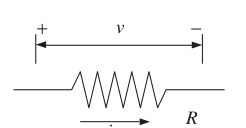
\includegraphics[width=0.9\textwidth]{Resistor}
        \caption{Στοιχείο αντίστασης}
    \end{minipage}\hfill
    \begin{minipage}{0.45\textwidth}
        \centering
        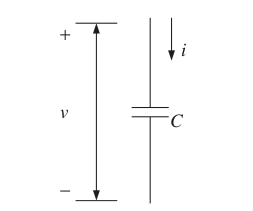
\includegraphics[width=0.9\textwidth]{Capacitor}
        \caption{Στοιχείο πυκνωτή}
    \end{minipage}
\end{figure}


Οι συναρτήσεις των στοιχείων ενος ηλεκτρικού κυκλώματος καθορίζουν αν το κύκλωμα θα είναι γραμμικό ή μη γραμμικό. Γραμμικό στοιχείο είναι το στοιχείο του οποίου η συνάρτηση δεν περιλαμβάνει συντελεστές στη δύναμη του 2 ή μεγαλύτερη.
Όταν ένα ηλεκτρικό κύκλωμα περιλαμβάνει μόνο στοιχεία γραμμικά τότε και το ίδιο το κύκλωμα είναι γραμμικό.

Στα πλαίσια της εργασίας, θα ασχοληθούμε αυστηρά μόνο με γραμμικά κυκλώματα τα οποία ακολουθούν την αρχή της επαλληλίας (\textlatin{superposition principle}).  Έτσι, η έξοδος ενός κυκλώματος $F(x)$,όταν εφαρμόζεται ένας γραμμικός συνδυασμός σημάτων $a_1x_1(t) + a_2x_2(t)$ ως είσοδος, θα ισούται με τον γραμμικό συνδυασμό των εξόδων των σημάτων $x_1(t)$ και $x_2(t)$ όταν αυτά εφαρμόζονται ξεχωριστά, δηλαδή:

\begin{equation}
    F\{a_1x_1(t) + a_2x_2(t)\} = a_1F\{x_1(t)\} + a_2F\{x_2(t)\}
\end{equation}


\subsection{Κυκλωματικά στοιχεία}

Με τον όρο κυκλωματικό στοιχείο στα πλαίσια της εργασίας μας, περιγράφουμε ηλεκτρικά στοιχεία με δύο τερματικά. Σαν γενικές κατηγορίες των στοιχείων αυτών έχουμε τα παθητικά και τα ενεργά στοιχεία. Τα ενεργά στοιχεία είναι αυτά που παρέχουν ηλεκτρική ενέργεια και δρουν ως πηγές ενός κυκλώματος. Οι πηγές που θα συναντήσουμε είναι ανεξάρτητες και έχουν την ιδιότητα ότι η τάση $v(t)$ ή το ρεύμα $i(t)$ που περνάει απο μέσα τους εκφράζεται ως εξής:
\begin{itemize}
    \item Ανεξάρτητη πηγή τάσης ορίζεται η πηγή της οποίας η τάση είτε είναι σταθερή ή μεταβάλεται σε συνάρτηση με τον χρόνο $v = f(t)$. 
    \item Ανεξάρτητη πηγή ρεύματος ορίζεται η πηγή της οποίας το ρεύμα είτε είναι σταθερό ή μεταβάλεται σε συνάρτηση με τον χρόνο $i = f(t)$.
\end{itemize}

Αντίθετα με τα ενεργά στοιχεία, τα παθητικά στοιχεία καταναλώνουν και δεν παράγουν ενέργεια. Η ενέργεια που καταναλώνουν τα παθητικά στοιχεία είτε θα μετατραπεί σε κάποιου άλλου είδους ενέργειας (για παράδειγμα θερμότητα) είτε θα αποθηκευτεί (σε ενέργεια ηλεκτρικού ή μαγνητικού πεδίου). Τονίζουμε ότι κατά την μετατροπή της ενέργειας, η ισχύς που υπολογίζουμε στην έξοδο δεν θα ενισχυθεί. Τα πιο γνωστά παθητικά στοιχεία είναι το πηνίο, η αντίσταση και ο πυκνωτής.

Αν δούμε τη μορφή της εξίσωσης που χαρακτηρίζει το κάθε στοιχείο μπορούμε να διαφοροποιήσουμε την κατηγοριοποίηση σε δύο ομάδες. Για αριθμό στοιχείων $m_1$ έχουμε την πρώτη ομάδα που έχει την παρακάτω μορφή εξίσωσης:

\begin{equation}
    i_k(t) = g_k u_k(t) + c_k \frac{du_k(t)}{dt} + s_k(t)
\end{equation}

Στην ομάδα αυτή έχουμε αντιστάτες, πυκνωτές και πηγές ρεύματος.

Αντίστοιχα, η δεύτερη ομάδα με αριθμό στοιχείων $m_2$ εκφράζεται από την παρακάτω μορφή εξίσωσης:

\begin{equation}
    u_k(t) = l \frac{\overrightarrow{d i_k}(t)}{dt} + \overrightarrow{s_k}(t)
\end{equation}

Στην δεύτερη ομάδα έχουμε πηνία και πηγές τάσης.

\subsection{Τροποποιημένη ανάλυση κόμβων}

Η συμπεριφορά ενός κυκλώματος περιγράφεται από ένα σύνολο εξισώσεων που σχηματίζεται συνδυάζοντας τις συναρτήσεις που προκύπτουν από τους νόμους του $Kirchoff$ για την τάση (\textlatin{Kirchoff's Voltage Law (KVL)} και το ρεύμα (\textlatin{Kirchoff's Current Law (KCL))}. Ορίζουμε τους παραπάνω νόμους ως εξής:

\begin{enumerate}
  \item Ο νόμος ρευμάτων του \textlatin{Kirchoff (KCL)}  μας λέει οτι το αλγεβρικό άθροισμα των ρευμάτων σε κάθε κόμβο ενός κυκλώματος ισούται με το μηδέν.
  \begin{equation}
    \label{4} \sum_{k=1}^{n}i_k(t) = 0 \Leftrightarrow A \overrightarrow{i}(t) = \overrightarrow{0}
  \end{equation}
  \item Ο νόμος τάσεων του \textlatin{Kirchoff(KVL)} μας λέει ότι σε κάθε κλειστό βρόγχο ενός κυκλώματος, το άθροισμα των τάσεων (διαφορών δυναμικού) των επιμέρους κλάδων που απαρτίζουν τον βρόγχο ισούται με το μηδέν.
  \begin{equation}
      \sum_{k=1}^{m}u_k(t) = 0 \Leftrightarrow \overrightarrow{u}(t) = A^T \overrightarrow{u}(t)
  \end{equation}
\end{enumerate}


Χρησιμοποιώντας τις συναρτήσεις που προκύπτουν από τους παραπάνω νόμους και ακολουθώντας τις κλασσικές μεθοδολογίες επίλυσης γραμμικών συστημάτων μπορούμε να βρούμε τη λύση για πολύ απλά συστήματα. Καταλαβαίνουμε όμως, με την κλασσική επίλυση των συστημάτων δεν μπορούμε να έχουμε κλιμάκωση στο μέγεθος των ηλεκτρικών κυκλωμάτων.

Για τον παραπάνω λόγο, μπορούμε να χρησιμοποιήσουμε την Τροποποιημένη Ανάλυση Κόμβων (\textlatin{Modified Nodal Analysis (MNA)}) για να λύσουμε με συστηματικό τρόπο συστήματα πολύ μεγάλης κλίμακας.

Τα βασικά βήματα για την Τροποποιημένη Ανάλυση Κόμβων είναι τα εξής:

\begin{enumerate}
    \item Γράφουμε με βάση τον Νόμο Ρεύματος του \textlatin{Kirchoff} την εξίσωση $Ai=0$ όπου $A$ είναι ο πίνακας μειωμένης πρόσπτωσης (\textlatin{reduced incidence matrix}) και το $i$ είναι διάνυσμα με όλα τα ρεύματα σε κάθε κλάδο
    \item Χρησιμοποιώντας τις εξισώσεις που περιγράφουν το κάθε κυκλωματικό στοιχείο, προσπαθούμε να εξαλείψουμε όσο το δυνατόν περισσότερες μεταβλητές ρεύματος με τη βοήθεια του Νόμου \textlatin{Kirchoff} για το ρεύμα. Με το βήμα αυτό καταλήγουμε να έχουμε εξισώσεις οι οποίες είναι σε συνάρτηση με την τάση $u = A^T v$.
    \item Στο βήμα αυτό, χρησιμοποιούμε τον Νόμο \textlatin{Kirchoff} για την τάση (\textlatin{Kirchoff's Voltage Law (KVL)}) και αντικαθιστούμε όλα τις τάσεις κλάδων με τάσεις κόμβων στη γείωση.
    \item Οι εξισώσεις στοιχείων των οποίων οι μεταβλητές τάσης δεν μπορούσαν να εξαλειφθούν, τις προσθέτουμε σαν επιπλέον εξισώσεις στο \textlatin{MNA} σύστημα.
\end{enumerate}

Με βάση τα παραπάνω βήματα καταλήγουμε στο εξής σύστημα ~\cite{ho1975modified}:
\begin{equation}
    \begin{bmatrix}
    Y & B\\
    C & Z
    \end{bmatrix}
    \begin{bmatrix}
    v\\
    i
    \end{bmatrix} = 
    \begin{bmatrix}
    s_v\\
    s_j
    \end{bmatrix}
\end{equation}


Όπου ισχύει η εξίσωση $Z_i + Y_u = s$ για $Z$ και $Y$ πίνακες ενώ $s$ είναι διάνυσμα.

% Οι παραπάνω εξισώσεις αφορούν αντίστοιχα τα στοιχεία των ομάδων 1 και 2.  ́Ετσι λοπόν
% προκύπτουν οι αντίστοιχες εξισώσεις:
% \begin{equation} \label{u1t}
%     \overrightarrow{u_1}(t) =  A^{T}_{1} \overrightarrow{u}(t)
% \end{equation}

% \begin{equation} \label{u2t}
%     \overrightarrow{u_2}(t) =  A^{T}_{2} \overrightarrow{u}(t)
% \end{equation}

% Αντίστοιχα, τώρα για τα στοιχεία των ομάδων 1 και 2, γράφουμε τις χακτηριστικές υπό την
% μορφή πινάκων:

% \begin{equation} \label{i1t}
%     \overrightarrow{i_1}(t) =  G \overrightarrow{u_1}(t) + C \frac{d \overrightarrow{u_1}(t)}{dt} + \overrightarrow{s_1}(t)
% \end{equation}

% \begin{equation} \label{u2t2}
%     \overrightarrow{u_2}(t) =  L \frac{d\overrightarrow{i_2}(t)}{dt} + \overrightarrow{s_2}(t)
% \end{equation}

% Επόμενο βήμα είναι η αντικατάσταση της εξίσωση \ref{u1t} στην εξίσωση \ref{i1t} και αντίστοιχα της εξίσωσης \ref{u2t} στην εξίσωση \ref{u2t2}. Μετά την αντίκατασταση προκύπτουν οι ακόλουθες εξισώσεις:

% \begin{equation} \label{A1GA}
%     A_1 G A^{T}_{1} \overrightarrow{u_1}(t) + A_1 C A^{T}_{1} \frac{d \overrightarrow{u_1}(t)}{dt} + A_2 \overrightarrow{i_2}(t) = - A_1 \overrightarrow{s_1} (t)
% \end{equation}

% \begin{equation} \label{AT2}
%     A^{T}_{2} \overrightarrow{u}(t) - L \frac{d \overrightarrow{i_1}(t)}{dt} = \overrightarrow{s_2}(t)
% \end{equation}

% Ο συνδυασμός των εξισώσεων \ref{A1GA} και \ref{AT2} δίνει ένα επεκταμένο (σύνθετο) σύστημα εξισώσεων διαστάσεων $[(n − 1) + m 2 ] × [(n − 1) + m 2 ]$, το οποίο το γράφουμε σε έναν ως εξής:
% \begin{center}
% \begin{bmatrix}
% A_1 G A^{T}_{1} & A_2\\
% A^{T}_{2} & 0
% \end{bmatrix} \begin{bmatrix}
% \overrightarrow{u_1}(t) \\
% \overrightarrow{i_2}(t)
% \end{bmatrix} + \begin{bmatrix}
% A_1 C A^{T}_{1} & 0\\
% 0 & -L
% \end{bmatrix} $\frac{d}{dt}$
% \begin{bmatrix}
% \overrightarrow{u_1}(t) \\
% \overrightarrow{i_2}(t)
% \end{bmatrix} = \begin{bmatrix}
% -A_1 \overrightarrow{s_1}(t) \\
% \overrightarrow{s_2}(t)
% \end{bmatrix}
% \end{center}


% Θέτοντας του πίνακες και τα διανύσματα ως:

% \begin{center}
% \widetilde{G} = \begin{bmatrix}
% A_1 G A_{1}^T & A_2 \\
% A_{2}^{T} & 0
% \end{bmatrix}, \widetilde{C} = \begin{bmatrix}
% A_1 C A_{1}^T & 0 \\
% 0 & -L
% \end{bmatrix}, \overrightarrow{x}(t) = \begin{bmatrix}
% \overrightarrow{u_1}(t) \\
% \overrightarrow{i_2}(t)
% \end{bmatrix}, \overrightarrow{e}(t) = \begin{bmatrix}
% -A_1\overrightarrow{s_1}(t) \\
% \overrightarrow{s_2}(t)
% \end{bmatrix}, 
% \end{center}

% λαμβάνουμε λαμβάνουμε τελικά, σε μια πιο ευδιάκριτη μορφή, ένα σύστημα γραμμικών διαφορικών εξισώσεων πρώτης τάξης με σταθερούς συντελεστές:

\begin{equation} \label{GxtCdxt}
\widetilde{G} \overrightarrow{x}(t) + \widetilde{C}\frac{d \overrightarrow{x}(t)}{dt} = \overrightarrow{e}(t) \Leftrightarrow \widetilde{G} \overrightarrow{x}(t) + \widetilde{C}\overrightarrow{x}(t) = \overrightarrow{e}(t)
\end{equation}

\section{Μεταβατική ανάλυση και ανάλυση συνεχούς}
Τα κυκλώματα στην πλειονότητα τους εκτός απο ανιστάτες περιλαμβάνουν και δυναμικά στοιχεία (πυκνωτές και πηνεία) τα οποία ανάλογα με τον χρόνο παρουσιάζουν μεταβολή.

Με βάση την παραπάνω παρατήρηση, η ανάλυση μας μπορεί με βάση τον χρόνο να οριστεί σε δυο κατηγορίες:
\begin{itemize}
    \item Ανάλυση συνεχούς: Σε αυτή την ανάλυση προσεγγίζουμε μια λύση του κυκλώματος για μια δεδομένη χρονική στιγμή.
    \item Μεταβατική ανάλυση: Αναφέρεται σε κυκλώματα με δυναμικά στοιχεία στα οποία μας ενδιαφέρει η απόκριση με βάση τον χρόνο.
\end{itemize}

\subsection{Ανάλυση συνεχούς}
Η παρούσα ανάλυση όπως τονίσαμε αναφέρεται σε συγκεκριμένες χρονικές στιγμές. Συνεπώς, υπολογίζουμε για διάφορα \textlatin{DC} σήματα την απόκριση που παρουσιάζει το κύκλωμα. Το χαρακτηριστικό της ανάλυσης είναι οτι λόγω της μη μεταβολής του χρόνου, έχουμε μηδενική χρονική παράγωγο για τις διεγέρσεις και τις αποκρίσεις.

Το σύστημα της εξίσωσης \ref{GxtCdxt} γίνεται:

\begin{equation}
    \begin{bmatrix}
        A_1 G A_1^T & A_2 \\
        A_2^T & 0
    \end{bmatrix}
    \begin{bmatrix}
        \overrightarrow{u_1} \\
        \overrightarrow{i_2}
    \end{bmatrix} = 
    \begin{bmatrix}
        -A_1 \overrightarrow{s_1} \\
        \overrightarrow{s_2}
    \end{bmatrix}
\end{equation}

Για την παραπάνω ανάλυση είναι σημαντικό να αναφερθούμε στους συμμετρικούς και θετικά ορισμένους πίνακες \textlatin{Symmetric and Positive Definite(SPD)} οι οποίοι παρουσιάζουν ιδιαίτερες ιδιότητες που μας βοηθούν για ταχύτερη επίλυση των συστημάτων. Για να προκύψουν τέτοιοι πίνακες είναι απαραίτητο το κύκλωμα να αποτελείται μόνο απο αντιστάσεις, πυκνωτές και πηγές ρεύματος. Όλα τα υπόλοιπα στοιχεία πρέπει να απουσιάζουν.

H συμμετρία \textlatin{symmetric} ενός πίνακα $A$ ορίζεται όταν ο πίνακας ισούται με τον αντίστροφο του, δηλαδή ισχύει $A(i, j) = A(j, i)$ για $i \neq j$.

\begin{equation}
A = A^T \Leftrightarrow A\ is\ symmetric, \forall A \in \mathbb{R} ^{nxn}
\end{equation}

Για την ιδιότητα του θετικά ορισμένου \textlatin{(positive definite)} πίνακα Α, είναι όταν η τετραγωνική μορφή είναι θετική για κάθε διάνυσμα εκτός του μηδενικού:

\begin{equation}
\overrightarrow{x}^T A \overrightarrow{x} > 0, \forall \overrightarrow{x} \in \mathbb{R}^{n}, \overrightarrow{x} \neq
 \overrightarrow{0} \Leftrightarrow A \ is \ positive\ definite
 \end{equation}

\subsection{Μεταβατική ανάλυση}

Αντίθετα με την ανάλυση συνεχούς (\textlatin{DC analysis}) όπου πραγματοποιείται η ανάλυση για συγκεκριμένες χρονικές στιγμές, στην μεταβατική ανάλυση \textlatin{Transient analysis} βασιζόμαστε στον υπολόγισμό της χρονικής απόκρισης του κυκλώματος για δεδομένες διεγέρσεις.


Αρχικά αναζητούμε επίλυση για το πρόβλημα των αρχικών τιμών στο οποίο για δεδομένο διάνυσμα διεγέρσεων ${e}(t)$ και θεωρώντας πως το διάνυσμα των αποκρίσεων ${x}(t)$ είναι καθορισμένο για μία δεδομένη χρονική στιγμή $t_0$ ως ${x}(t_0)$ = ${x_0}$ (αρχική συνθήκη),
έχουμε:

\[
\begin{cases}
    \widetilde{G} {x}(t) + \widetilde{C}\dot{{x}}(t) = {e}(t) \\
     {x}(t_0) = {x_0}
\end{cases}
\]

έχει μοναδική λύση ${x}(t)$ (υπό ορισμένες συνθήκες) σε ένα διάστημα $[t_0 , t_f]$ σε διακριτούς χρόνους $t_0 < t_1 < t_2 < ... < t_m = t_f$.

% Αρχικά αναζητούμε επίλυση για το πρόβλημα των αρχικών τιμών στο οποίο για δεδομένο διάνυσμα διεγέρσεων $\overrightarrow{e}(t)$ και θεωρώντας πως το διάνυσμα των αποκρίσεων $\overrightarrow{x}(t)$ είναι καθορισμένο για μία δεδομένη χρονική στιγμή $t_0$ ως $\overrightarrow{x}(t_0)$ = $\overrightarrow{x_0}$ (αρχική συνθήκη),
% έχουμε:

% \[
% \begin{cases}
%     \widetilde{G} \overrightarrow{x}(t) + \widetilde{C}\dot{\overrightarrow{x}}(t) = \overrightarrow{e}(t) \\
%      \overrightarrow{x}(t_0) = \overrightarrow{x_0}
% \end{cases}
% \]

% έχει μοναδική λύση $\overrightarrow{x}(t)$ (υπό ορισμένες συνθήκες) σε ένα διάστημα $[t_0 , t_f]$ σε διακριτούς χρόνους $t_0 < t_1 < t_2 < ... < t_m = t_f$.

Οι παρακάτω προσεγγίσεις μας βοηθάνε στο πρόβλημα της εύρεσης των αρχικών τιμών (\textlatin{Initial Value Problem (IVP)}:

\begin{enumerate}
  \item Προσέγγιση \textlatin{Backward Euler (BE)} ή \textlatin{Implicit Euler (IE)}\\
        Σύμφωνα με αυτήν και για μονοδιάστατη περίπτωση, γράφουμε μια \textlatin{Taylor} εκτεταμένη σειρά στο $t_{n+1}$ και έχουμε:\\
        \begin{equation}
            x(t) = x(t_{n+1}) + (t - t_{n+1}) x'(t_{n+1}) + \frac{(t - t_{n+1})^2}{2}x''(\xi)
        \end{equation}
        για κάποιο \xi μεταξύ $t_{n+1})$ και $t$. Τότε, για $t = t_n = t_{n+1} - h$ έχουμε:
        \begin{equation}
            x(t_n) = x(t_{n+1}) h x'(t_{n+1}) + \frac{h^2}{2}x''(\xi)
        \end{equation}
        Για πολυδιάστατο $m$ χώρο έχουμε:
        \begin{equation}
            x(t_n) = x_n + h f(x_{n+1}, t_{n+1}) => x_{n+1} = x_n + hf_{n+1}
        \end{equation}
 \item Προσέγγιση \textlatin{Trapezoidal Rule(TR)}\\
    Για ακόμη καλύτερη προσέγγιση στη λύση μας, χρειάζεται να καταφύγουμε σε μεθόδους υψηλότερης τάξης. Μια τέτοια μέθοδος είναι η \textlatin{Trapezoidal Rule(TR)}. Για μονοδιάσ`τατη περίπτωση χρησιμοποιούμε μια \textlatin{Taylor} εκτεταμένη σειρά στο $t_{n+1}$ και έχουμε:
    
    \begin{equation} \label{tr1}
      x(t) = x(t_n) + (t - t_n) x'(t_n) + \frac{(t - t_n)^2}{2}x''(t_n) + \frac{t - t_n)^3}{6} x'''(\xi)
    \end{equation}
    
    για κάποιο \xi μεταξύ $t_n$ και $t_{n+1}$ το οποίο μπορούμε να παραγοντοποιήσουμε και να λάβουμε:
    
    \begin{equation} \label{tr2}
      x'(t) = x'(t_n) + (t - t_n) x''(t_n) + \frac{(t - t_n)^2}{2}x'''(\xi)
    \end{equation}
    
    γράφοντας τα δύο αποτελέσματα απο τις \ref{tr1} και \ref{tr2} και για $t = t_{n+1} = t_n + h$, πολλαπλασιάζουμε την πρώτη ισότητα με 2 και την δεύτερη με $-h$ για να λάβουμε:
    
    \begin{equation}
      2x'(t_{n+1}) = 2x'(t_n) + 2h x'(t_n) + h^2 x''(t_n) + \frac{h^3}{3}x'''(\xi)
    \end{equation}
    
    \begin{equation}
      -h x'(t_{n+1}) = -h x'(t_n) - h^2 x''(t_n) - \frac{h^3}{2}x'''(\xi)
    \end{equation}
    
    Προσθέτοντας τις δύο ισότητες και διαιρώντας με το 2 παίρνουμε:
    \begin{equation}
        x(t_{n+1}) - x(t_n) = \frac{h}{2} [ x'(t_{n+1}) + x'(t_n)] - \frac{h^3}{12} x'''(\xi)
    \end{equation}
    
    Για $m$ διαστάσεις, μπορούμε να γράψουμε την παραπάνω ισότητα ως:
    
    \begin{equation}
        x(t_{n+1}) - x(t_n) = \frac{h}{2} [x'(t_{n+1}) + x'(t_n)] + 0(h^3)
    \end{equation}
    
    Καταλήγουμε στον \textlatin{Trapezoidal Rule (TR)}:
    \begin{equation}
        x_{n+1} = x_n + \frac{h}{2} [ f(x_{n+1}, t_{n+1}) + f(x_n, t_n)]
    \end{equation}
    
    ή πιο απλά:
    
    \begin{equation}
        x_{n+1} = x_n + \frac{h}{2} (f_{n+1} + f_n)
    \end{equation}
    
    
\end{enumerate}

Σημειώνουμε οτι μεταξύ των δυο παραπάνω προσεγγίσεων, η μέθοδος \textlatin{Trapezoidal Rule (TR)} είναι η πιο συχνά χρησιμοποιούμενη μέθοδος για την προσομοίωση κυκλωμάτων. Επίσης, προσεγγίζει τη λύση καλύτερα και με μεγαλύτερη ακρίβεια την πραγματική λύση $x_n$ για τις διακριτές στιγμές $t_n$. Ένα ακόμη πλεονέκτημα της $TR$ έναντι της $BE$ είναι μπορούμε να έχουμε μεγαλύτερα βήματα στο χρόνο και σε δειγματοληψία η οποία είναι μεταβλητή.
\chapter{Μαθηματικό Υπόβαθρο}
\label{ch:3.chapterMathBackground}

\section{Αραιοί Πίνακες στα Γραμμικά Συστήματα}

Με το όρο Αραιοί Πίνακες \textlatin{(Sparse Matrices)} αναφερόμαστε σε πίνακες όπου τα περισσότερα στοιχεία τους είναι 0. Για την επιστήμη της πληροφορικής, οι πίνακες αυτοί έχουν ιδιαίτερο ενδιαφέρον καθώς μας δίνουν την δυνατότητα να συμπιέσουμε την πληροφορία που περιέχουν σε μικρότερο χώρο από ότι θα χρειάζονταν ένας πυκνός \textlatin{(dense)} πίνακας. Επίσης, μπορούμε να εκμεταλλευτούμε την ιδιότητα που έχουν οι πίνακες αυτοί και να προσεγγίσουμε μια λύση του γραμμικού συστήματος πιο γρήγορα απο ότι θα κάναμε σε έναν πυκνό \textlatin{(dense)} πίνακα.

\subsection{Αποθήκευση και απεικόνιση Αραιών Πινάκων}

Όπως τονίσαμε, η ιδιότητα των αραιών πινάκων να έχουν τα περισσότερα στοιχεία τους 0, μας δίνει την δυνατότητα να εφαρμόσουμε πιο αποτελεσματικούς τρόπους αποθήκευσης από το να κρατούσαμε όλα τα στοιχεία (μηδενικά και μη μηδενικά) στη μνήμη.

Υπάρχουν διάφοροι τρόποι αποθήκευσης. Στα πλαίσια της διπλωματικής και λόγω της εξωτερικής βιβλιοθήκης που χρησιμοποιούμε, θα σταθούμε σε 2 βασικές μεθόδους απεικόνισης των αραιών πινάκων.

\subsubsection{Τρίδυμη Δομή Απεικόνισης} \label{TripletForm}
Η δομή αυτή~\cite{davis2006direct} αποτελεί τον πιο απλό τρόπο απεικόνισης των αραιών πινάκων σε ένα υπολογιστικό σύστημα. Για κάθε μη μηδενικό στοιχείο του πίνακα, κρατάμε την γραμμή, τη στήλη και τη τιμή του στοιχείου.

Εκ πρώτης όψεως θα μπορούσε να παρατηρήσει κάποιος ότι χρειαζόμαστε 3 στοιχεία στη μνήμη μας για να απεικονίσουμε ένα μη μηδενικό στοιχείο. Δεν είναι όσο αποδοτικό όσο η απλή απεικόνιση που έχουμε για έναν πυκνό πίνακα όπου κρατάμε όλα τα στοιχεία στη μνήμη.

Το σημαντικό στοιχείο στην απεικόνιση ενός αραιού πίνακα είναι ότι τα στοιχεία που θα χρειαστεί να αποθηκεύσουμε θα είναι πολύ λιγότερα από το μέγιστο αριθμό στοιχείων που μπορεί να έχει ένας πίνακας μεγέθους $n x m$.


Παράδειγμα απεικόνισης αραιού πίνακα σε Τρίδυμη Δομή\\

\selectlanguage{english}
\begin{figure}[ht]
\centering
$\begin{matrix}
0 & 0 & 11.0\\
0 & 3 & 14.0\\
0 & 5 & 16.0\\
1 & 1 & 22.0\\
1 & 3 & 25.0\\
1 & 5 & 26.0\\
2 & 2 & 33.0\\
2 & 3 & 34.0\\
2 & 5 & 36.0\\
3 & 0 & 41.0\\
3 & 2 & 43.0\\
3 & 3 & 44.0\\
3 & 5 & 46.0
\end{matrix}$
\end{figure}
\selectlanguage{greek}

\\
Κάθε γραμμή του παραπάνω πίνακα έχει την παρακάτω μορφή:\\
\textlatin{I J A(I, J)}\\
όπου τα \textlatin{I} και \textlatin{J} είναι οι δείκτες για τον \textlatin{x} και \textlatin{y} άξονα αντίστοιχα και είναι με βάση το 0.

\subsubsection{Δομή της Συμπιεσμένης Στήλης \textlatin{Compressed Column Storage (CCS)}} \label{CCS}
Η δομή αυτή αποτελεί τον πιο συνηθισμένο τρόπο απεικόνισης ενός αραιού πίνακα σε ένα υπολογιστικό σύστημα. Η δομή αυτή αναφέρεται και ως \textlatin{Harwell-Boeing} απεικόνιση~\cite{duff1989sparse}. Σε σχέση με την Τρίδυμη Δομή Απεικόνισης, προσφέρει τη δυνατότητα να αποθηκεύσουμε μόνο τα μη μηδενικά στοιχεία ενός αραιού πίνακα, αλλά χωρίς να χρειαζόμαστε 3 στοιχεία της μνήμης για την απεικόνιση ενός στοιχείου του πίνακα.
Συνολικά για την απεικόνιση ενός αραιού πίνακα Α στη μορφή Συμπιεσμένης Στήλης \textlatin{(CCS)} χρειαζόμαστε 3 διαφορετικούς μονοδιάστατους πίνακες:
\begin{itemize}
  \item Πίνακας Τιμών: περιέχει τις τιμές του πίνακα
  \item Πίνακας Δεικτών των γραμμών: Περιέχει τους δείκτες για όλες τις γραμμές που υπάρχουν μη μηδενικά στοιχεία
  \item Πίνακας Δεικτών Στηλών: Στον πίνακα αυτό βρίσκονται οι δείκτες για τα στοιχεία στον Πίνακα τιμών που ξεκινάει μια στήλη του πίνακα Α. 
\end{itemize}

\subsection{Αλγοριθμική επίλυση αραιών πινάκων}
Η επίλυση αραιών πινάκων μπορεί να πραγματοποιηθεί είτε με την χρήση άμεσων επιλύσεων \textlatin{(direct solvers)} είτε με τη χρήση επαναληπτικών μεθόδων.

Οι μέθοδοι που χρησιμοποιούνται για την άμεση επίλυση γραμμικών συστημάτων που χρησιμοποιούν αραιούς πίνακες βασίζονται στην απαλοιφή κατά \textlatin{Gauss}.

Τα τελευταία χρόνια έχει εδραιωθεί η επίλυση γραμμικών συστημάτων αραιών πινάκων με τη χρήση επαναληπτικών μεθόδων. Οι μέθοδοι αυτοί επιτυγχάνουν την γρηγορότερη και πιο αποδοτική επίλυση των γραμμικών συστημάτων με τη χρήση των παρακάτω μεθοδολογιών:
Μετάθεση των εξισώσεων και των αγνώστων έτσι ώστε να εγγυηθούμε μια σταθερή \textlatin{LU} αποσύνθεση του πίνακα
Οργάνωση των υπολογισμών με βάση τη διαθέσιμη υπολογιστική ισχύ του υλικού \textlatin{(hardware)} στο οποίο πραγματοποιείται η επίλυση. Τα τελευταία χρόνια έχει εδραιωθεί η χρήση πολυνηματικών υπολογιστικών μονάδων από τη μεριά του επεξεργαστή αλλά και της κάρτας γραφικών (με τη χρήση τεχνολογιών τύπου \textlatin{CUDA, OpenCL}) που επιτρέπουν τη μαζική και παράλληλη επίλυση γραμμικών συστημάτων.

\section{Μέθοδοι Παραγοντοποίησης Πινάκων}

Η βασική μέθοδος επίλυσης ενός συστήματος γραμμικών εξισώσεων $Ax = b$ είναι ο πολλαπλασιασμός του δεξιού μέλους με τον αντίστροφο $x = A^Tb$ (όταν ο $A$ έχει ορθογώνιες στήλες). Ο περιορισμός της ορθογωνικότητας των στηλών καθώς και η μη αποδοτική επίλυση του συστήματος, καθιστά την απλή αυτή λύση μη βιώσιμη για γραμμικά συστήματα που συναντάμε σε πραγματικά προβλήματα.

Ένα βασικό εργαλείο για την επίλυση γραμμικών συστημάτων (ή για την προσέγγιση μιας λύσης) είναι η παραγοντοποίηση ενός πίνακα. Η βασική αρχή της παραγοντοποίησης είναι η αποσύνθεση ενός πίνακα σε γινόμενο από πίνακες. Ανάλογα με την εκάστοτε μέθοδο παραγοντοποίησης, οι επιμέρους πίνακες έχουν και διαφορετικές ιδιότητες τις οποίες μπορούμε να αξιοποιήσουμε κατά την επίλυση του γραμμικού συστήματος.

Η πιο βασική μέθοδος παραγοντοποίησης είναι η απαλοιφή κατά \textlatin{Gauss}. Η απαλοιφή αυτή μπορεί να εφαρμοστεί σε αντιστρέψιμους πίνακες όπου ο $A$ μετατρέπεται σε έναν άνω τριγωνικό U πίνακα ή παραγοντοποιείται σε ένα γινόμενο πινάκων $LU$ όπου $L$ είναι ο κάτω τριγωνικός και $U$ ο άνω τριγωνικός. Η μέθοδος αυτή αν και πολύ διαδεδομένη και χρήσιμη, έχει σαν βασικό μειονέκτημα οτι μπορεί να είναι "ασταθής" για ορισμένα γραμμικά συστήματα. Επίσης, είναι δύσκολο να προσδιορίσουμε το σφάλμα που έχει προκύψει κατά την παραγοντοποίση.

Τα παραπάνω προβλήματα που εμφανίζει η απαλοιφή κατά \textlatin{Gauss} έρχεται να αντιμετωπίσει η Μέθοδος Παραγοντοποίησης $QR$.

Στα πλαίσια των αλγορίθμων που θα αναλύσουμε, γίνεται χρήση της $QR$ παραγοντοποίησης η οποία μπορεί να επιτευχθεί με τη χρήση διάφορων μεθόδων.

Η $QR$ παραγοντοποίηση χρησιμοποιείται κυρίως για την επίλυση γραμμικών συστημάτων, προβλήματα με ιδιοτιμές και προσέγγιση λύσης με βάση την μέθοδο ελαχίστων τετραγώνων.

\subsubsection{Μέθοδος Παραγοντοποίησης \textlatin{QR}}

Ορίζουμε την Παραγοντοποίηση $QR$ ως εξής:\\

\selectlanguage{english}
\theoremstyle{definition}
\begin{definition}{QR}
\selectlanguage{greek}
Για πίνακα $Α$ διαστάσεων $m * n$ όπου $m >= n$ και έχει γραμμικά
ανεξάρτητες στήλες. Τότε υπάρχει ένας μοναδικός $m * n$ πίνακας $Q$ με $Q^TQ=D$,
$D=diag(d_1 ,...,d_n),  d_k >0, k=1,...,n$ και ένας μοναδικός άνω τριγωνικός πίνακας $R$ με
$r_kk =1, k=1,2,...,n$ έτσι ώστε $A=QR$

Η Παραγοντοποίηση $QR$ θα δούμε στην συνέχεια ότι αποτελεί βασικό στοιχείο στον $EBA$ αλγόριθμο καθώς χρησιμοποιείται σε κάθε επαναληπτικό βήμα.


\subsubsection{Επίλυση Παραγοντοποίησης QR με χρήση \textlatin{Householder} μεθόδου} \label{HouseholderMethod}

Η χρήση \textlatin{Householder} μεθόδου μας δίνει τη δυνατότητα να επιλύσουμε το ζητούμενο γραμμικό σύστημα πετυχαίνοντας μίκροτερες αποκλίσεις στα αποτελέσματα σε κάθε βήμα με αποτέλεσμα να αποφύγουμε την εύρεση $Q$ πίνακα ο οποίος δεν είναι ορθογώνιος ~\cite{trefethen1997numerical}.

Η ιδέα πίσω απο την μέθοδο \textlatin{Householder} είναι να σχεδιάσουμε επαναληπτικά πίνακες $Q_1,...,Q_n$ οι οποίοι σταδιακά μετατρέπουν τον $A$ πίνακα σε άνω τριγωνικό πίνακα:

\selectlanguage{english}
A = \begin{bmatrix}
x & x & x\\
x & x & x\\
x & x & x\\
x & x & x\\
\end{bmatrix} \quad \rightarrow \quad $ Q_1A$ = A = \begin{bmatrix}
x & x & x\\
0 & x & x\\
0 & x & x\\
0 & x & x\\
\end{bmatrix}  \quad \rightarrow  \quad $Q_2Q_1A$ = A = \begin{bmatrix}
x & x & x\\
0 & 0 & x\\
0 & 0 & x\\
0 & 0 & x\\
\end{bmatrix}  \quad \rightarrow \quad 

\begin{center}
$Q_3Q_2Q_1A$ = A = \begin{bmatrix}
x & x & x\\
0 & 0 & x\\
0 & 0 & x\\
0 & 0 & 0\\
\end{bmatrix}
\end{center}
\selectlanguage{greek}


όπου $x$ είναι μια μηδενική τιμή. Σημειώνουμε οτι ο $Q_k$ χρησιμοποιεί τις γραμμές $k:m$ και δεν πειράζει καθόλου τις πρώτες $k - 1$ γραμμές και στήλες. 
Συνεπώς η μορφή του πίνακα $Q$ κατα την επανάληψη $k$ θα είναι η εξής:

\[Q_k = \begin{bmatrix}
Ι_{κ-1} & 0 \\
0 & F \\
\end{bmatrix}\]

όπου $I_{k-1}$ είναι ένας $(k-1) * (k-1)$ μοναδιαίος πίνακας και ο $F$ έχει την εξής ιδιότητα:

\[Fx = \| x \|e_1\]

έτσι ώστε να εισαγάγει μηδενικά στο κάτω μέρος της στήλης $k$.

Ο πίνακας $F$ καλείται και \textlatin{Housholder} ανακλαστήρας (\textlatin{Housholder reflector})

Για $u = \|x\|e_1 - x$ και $P = \frac{uu^*}{u^*u}$ τότε έχουμε:

\[F = I - 2P = I - 2\frac{uu^*}{u^*u}\]

Για το $u$ επιλέγουμε το εξής:

\[u = x + sign(x(1))\|x\|e_1\]

Κατά την ολοκλήρωση της μεθόδου, ο πίνακας $A$ περιέχει τον πίνακα $R$ της Παραγοντοποίησης $QR$ και τα διανύσματα $u_1, ..., u_n$ είναι τα διανύσματα αντανάκλασης τα οποία θα χρησιμοποιηθούν επαναληπτικά για να σχηματίσουμε το $Q*b$ σε ένα γραμμικό σύστημα. 

\section{Χρήση προρυθμιστών με χρήση επαναληπτικών μεθόδων επίλυσης}

Κατά την επίλυση μεγάλης κλίμακας γραμμικών συστημάτων με τη χρήση επαναληπτικών μεθόδων προτείνεται η χρήση προρυθμιστών έτσι ώστε να επιτευχθεί γρηγορότερη και πιο αποδοτική λύση.

Υπάρχουν επιλύσεις οι οποίες δεν χρησιμοποιούν προρυθμιστές αλλά δεν είναι ανταγωνιστικοί και βιώσιμοι σε προβλήματα μεγάλης κλίμακας που βρίσκουμε σε πραγματικά προβλήματα. Μια τέτοια επίλυση είναι η Επαναληπτική Υπερχαλάρωση\textlatin{(Successive Overralaxation (SOR))}~\cite{young1954iterative} μέθοδος η οποία αποτελεί προσέγγιση της \textlatin{Gauss–Seidel (Liebmann)}. Στη μέθοδο αυτή για γραμμικό σύστημα
\[Ax = b\]
					
Χωρίζουμε τον πίνακα Α σε τρεις(3) υποπίνακες
\[Α = D + L + U\]

όπου 

\begin{itemize}
  \item $A$: περιέχει τις τιμές του πίνακα
  \item $D$ : Πίνακας που περιλαμβάνει μόνο τη διαγώνιο του Α
  \item $L$ : Κάτω τριγωνικός πίνακας που περιλαμβάνει όλα τα στοιχεία απο τη διαγώνιο και κάτω του πίνακα $Α$
  \item $U$ : Άνω τριγωνικός πίνακας που περιλαμβάνει όλα τα στοιχεία απο τη διαγώνιο και πάνω
\end{itemize}

Για την επίλυση του συστήματος χρησιμοποιούμε επαναληπτική μέθοδο που αξιοποιεί τιμές του $x$ από προηγούμενο βήμα για την εύρεση του $x$ στο τρέχον βήμα.

Οι πιο σύγχρονες μέθοδοι που χρησιμοποιούνται για την επίλυση μεγάλης κλίμακας γραμμικά συστήματα χρησιμοποιούν προρυθμιστές υποχωρου \textlatin{Krylov}. 

\section{Υποχώροι \textlatin{Krylov}} \label{KrylovSubspaces}

Οι υποχώροι \textlatin{Krylov} εμφανίζονται σε πολλές επαναληπτικές μεθόδους για την επίλυση γραμμικών συστημάτων αραιών πινάκων. 

Μπορούμε να ορίσουμε τους υποχώρους \textlatin{Krylov} ώς εξής:


\selectlanguage{english}
\theoremstyle{definition}
\begin{definition}{Krylov}
\selectlanguage{greek}
Για μη-αντιστρέψιμο πίνακα $A \in C^{NxN}$ και  $y \neq 0 \in C^{N}$ o Ν-οστος \textlatin{Krylov} (υπο)χώρος $K_{n}(A,y)$ που παράγεται απο τον $Α$ στον $y$ είναι
\[ Κ_{n} := K_{n}(A,y) := span(y,Ay,...,A^{n-1}y) \]


Χαρακτηριστικά που μπορούμε να παρατηρήσουμε στον παραπάνω ορισμό είναι τα παρακάτω:
\[Κ_1 \subseteq  K_2 \subseteq  K_3 \subseteq ... \]
Οι διαστάσεις αυξάνονται κατά μια σε κάθε βήμα.
\end{definition}

\selectlanguage{greek}
\chapter{Μέθοδοι Υποβιβασμού Τάξης Μοντέλου}
\label{ch:4.chapterMOR}

Όπως τονίσαμε και στην εισαγωγή της διπλωματικής εργασίας (\ref{ch:1.chapterIntroduction}) τα κυκλώματα που εμφανίζονται σε πραγματικές εφαρμογές έχουν φτάσει τα εκατομμύρια στοιχεία. Τα γραμμικά συστήματα που προκύπτουν από τέτοιας κλίμακας κυκλώματα καθιστούν την συμβατική επίλυση αδύνατη.

Μια από τις πλέον εδραιωμένες τεχνικές για τη μείωση της πολυπλοκότητας των γραμμικών κυκλωμάτων οι οποίες αποσκοπούν στη μείωση των απαιτούμενων υπολογισμών ή στην απλοποίηση των μαθηματικών μοντέλων είναι οι μέθοδοι υποβιβασμού τάξης μοντέλου. (\textlatin{Model Order Reduction (MOR)}).

Οι μέθοδοι υποβιβασμού τάξης μοντέλου που θα εξετάσουμε στα πλαίσια της παρούσας διπλωματικής εργασίας βασίζονται στους υποχώρους \textlatin{Krylov} ~\ref{KrylovSubspaces}. Τέτοιες μέθοδοι αποτελούν οι \textlatin{Passive Reduced-order Interconnect Macromodeling Algorithm (PRIMA)}~\cite{odabasioglu2003prima} και \textlatin{ Structure-Preserving Reduced-order Interconnect Macromodeling (SPRIM)} ~\cite{freund2004sprim}


\section{Η μέθοδος υποβιβασμού τάξης μοντέλου \textlatin{PRIMA}}

Ο πλεόν βασικός αλγόριθμος για υποβιβασμό τάξης μοντέλου \textlatin{MOR} είναι ο \textlatin{Passive Reduced-order Interconnect Macromodeling Algorithm (PRIMA)}. Μέρος του αλγορίθμου είναι και η μέθοδος \textlatin{Block Arnoldi} που θα εξετάσουμε και υλοποιήσαμε στα πλαίσια της διπλωματικής εργασίας. O \textlatin{Block Arnoldi} αλγόριθμος χρησιμοποιείται για την παραγωγή ορθοκανονικής βάσης για έναν πίνακα μετασχηματισμού.

Πρίν περιγράψουμε τον αλγόριθμο \textlatin{PRIMA} ορίζουμε τους πίνακες οι οποίοι προκύπτουν από τη μέθοδο \textlatin{MNA}:

\begin{equation} \label{Cxn}
    C x_n = -G x_n + B v_p
\end{equation}
\[
    i_p = L^T x_n
\]
όπου τα διανύσματα $i_p$ και $v_p$ δηλώνουν τις πηγές ρεύματος και τάσης αντίστοιχα
\[
    G = 
    \begin{bmatrix}
    N & E \\
    -E^T & 0
    \end{bmatrix}\\
\]
\[
    C = 
    \begin{bmatrix}
    Q & 0 \\
    0 & H
    \end{bmatrix}\\
\]
\[
    x_n = 
    \begin{bmatrix}
    v \\
    i
    \end{bmatrix}\\
\]

Οι $n * n$ πίνακες $G$ και $C$ αντιπροσωπεύουν τους πίνακες αγωγιμότητας και επιδεκτικότητας. Οι $N$
, $Q$ και $H$ πίνακες περιλαμβάνουν τις αντιστάσεις, πυκνωτές και πηνία αντίστοιχα. Ο πίνακας $E$ περιλαμβάνει μονάδες, αρνητικές μονάδες και μηδενικά που αντιστοιχούν στις μεταβλητές ρεύματος των νόμων του  \textlatin{Kirchhoff (KCL)}. Στην περίπτωση που οι N-θύρες του κυκλώματος περιλαμβάνουν μόνο θετικά γραμμικά στοιχεία, $Q$, $H$ και $N$ είναι συμμετρικοί, θετικά δηλωμένοι πίνακες (\textlatin{Symmetric Positive Definite (SPD)}). Με βάση το παραπάνω ο $C$ είναι επίσης \textlatin{SPD}. 

Συνεπώς, επιστρέφοντας στην ισότητα \ref{Cxn}, δηλώνουμε:

\begin{equation}
    A = -G^{-1}C
\end{equation}
\begin{equation}
    R = G^{-1}B
\end{equation}


Μετά από $\left\lfloor\dfrac{q}{N}\right\rfloor +1$ επαναλήψεις (η επιπλέον επανάληψη είναι απαραίτητη μόνο όταν $\frac{q}{N}$ δεν είναι ακέραιος) του \textlatin{PRIMA}, o $n x q$ πίνακας $X$ είναι ο εξής:

\[
    colsp(X) = K_r(A, R,\left\lfloor\dfrac{q}{N}\right\rfloor)
\]
\[
    X^T X = I_q
\]

Στον βασικό αλγόριθμο \textlatin{PRIMA} χρησιμοποιείται μια παραλλαγή της μεθόδου \textlatin{Block Arnoldi} η οποία μας δίνει το εξής:
\[
    (X^T C X)\dot{\widetilde{x_q}} = - (X^T G X)\dot{\widetilde{x_q}} + (X^T B)u_p
\]
\[
    i_p = (L^TX)\dot{\widetilde{x_q}}
\]

Το υποβιβασμένης τάξης μοντέλο των \textlatin{MNA} πινάκων είναι:

\[
    \widetilde{C} = X^T C X
\]
\[
    \widetilde{G} = X^T G X
\]
\[
    \widetilde{B} = X^T B
\]
\[
    \widetilde{L} = X^T L
\]

Μετά τον υποβιβασμό του μοντέλου του πίνακα $Y(s)$ στο οποίο αναφερόμαστε ως $\hat{Y}(s)$ είναι πλέον:
\[
    \hat{Y}(s) = \widetilde{L}^T (\widetilde{G} + s \widetilde{C})^{-1} \widetilde{B}
\]

Τυπικά, το μέγεθος των πινάκων $\widetilde{G}$ και $\widetilde{C}$ είναι μικρό με αποτέλεσμα αν είναι εύκολο να βρούμε τους πόλους και τα μηδενικά του $\hat{Y}(s)$.

\section{Η μέθοδος υποβιβασμού τάξης μοντέλου \textlatin{SPRIM}}

Για την περιγραφή του αλγορίθμου \textlatin{SPRIM} θα χρειαστεί να ορίσουμε τους εξής πίνακες:

\[
   G = 
    \begin{bmatrix}
    G_1  & G^T_2\\
    -G_2 & 0
    \end{bmatrix}
\]
\[
    C = 
    \begin{bmatrix}
    C_1  & 0\\
    0 & C_2
    \end{bmatrix}
\]
\[
    B = 
    \begin{bmatrix}
    B_1\\
    0
    \end{bmatrix}
\]

Στο πρώτο βήμα του αλγορίθμου, δημιουργούμε τους εξής πίνακες $A$ και $R$ ως εξής:
\[
    A = (G + sC)^{-1}C
\]
\[
    R = (G + sC)^{-1}B
\]

Στη συνέχεια και ένα από τα βασικά σημεία του αλγορίθμου είναι η επιλογή της μεθόδου για την παραγωγή του υπο-χώρου \textlatin{Krylov}. Το σημείο αυτό είναι που εισέρχεται και η μελέτη που πραγματοποιήσαμε στα πλαίσια της διπλωματικής εργασίας για την χρήση του Εκτεταμένου \textlatin{Block Arnoldi} αλγορίθμου \ref{EBA}.

Με τη χρήση του επιθυμητού αλγορίθμου λαμβάνουμε το εξής αποτέλεσμα:

\[
    span(V_n) = K_n(A, R)
\]

Συνεχίζουμε με το επόμενο βήμα να είναι ο κατακερματισμός του πίνακα $V_n$ σε κομμάτια (\textlatin{blocks}):

\[
V_n = \begin{bmatrix}
V_1 \\
V_2
\end{bmatrix}
\]

o οποίος μετατρέπεται στην εξής μορφή:

\[
V_n = \begin{bmatrix}
V_1 & 0 \\
0 & V_2
\end{bmatrix}
\]

Υπολογίζουμε τους νέους πίνακες μέσω της ελαχιστοποίησης:

\[
    \widetilde{G_1} = V_q^{T}G_1V_1
\]
\[
    \widetilde{G_2} = V^2_TG_2V_1
\]
\[
    \widetilde{C_1} = V^1_TC_1V_1
\]
\[
    \widetilde{C_2} = V^2_TC_2V_2
\]
\[
    \widetilde{B_1} = V^1_TB_1
\]

και με βάση του πίνακες αυτούς έχουμε:


\[
\widetilde{G_n} = \begin{bmatrix}
\widetilde{G_1} & \widetilde{G_2}^T \\
-\widetilde{G_2}^T & 0
\end{bmatrix}
\]
\[
\widetilde{C_n} = \begin{bmatrix}
\widetilde{C_1} & 0 \\
0 & \widetilde{C_2}
\end{bmatrix}
\]
\[
\widetilde{B_n} = \begin{bmatrix}
\widetilde{B_1} \\
0
\end{bmatrix}
\]

Τέλος, από τους νέους πίνακες υπολογίζεται η συνάρτηση μεταφοράς του συστήματος με
τον εξής τρόπο:
\begin{equation}
    \Tilde{Z_n}(s) = \Tilde{B_n}^T(\Tilde{G_n} + s\Tilde{C_n})^{-1}\Tilde{B_n}
\end{equation}

\include{5.chapterAlgorithms}
\selectlanguage{greek}
\chapter{Πειραματική Διαδικασία}
\label{ch:6.chapterImplementation}

\section{Περιγραφή της πειραματικής διαδικασίας}
Στόχος της πειραματικής διαδικασίας είναι η εφαρμογή των μεθόδων υποβιβασμού τάξης μεγέθους και η χρήση εκτεταμένων υποχώρων \textlatin{Krylov} σε πραγματικά κυκλώματα μεσαίας και μεγάλης κλίμακας. 

Μέσω της τροποποιημένης ανάλυσης κόμβων μετατρέπουμε τα δίκτυα τροφοδοσίας ολοκληρωμένων συστημάτων σε γραμμικά συστήματα στα οποία θα εφαρμόσουμε τον \textlatin{Extended Block Arnoldi (EBA)} αλγόριθμο για να πετύχουμε υποβιβασμό της τάξης μεγέθους και τελικά επίλυση των συστημάτων.

Τα πραγματικά κυκλώματα που θα μελετήσουμε είναι τα δίκτυα τροφοδοσίας των ολοκληρωμένων κυκλωμάτων της ΙΒΜ.

Σαν οδηγό στην υλοποίηση μας χρησιμοποιούμε το εργαλείο \textlatin{MATLAB} το οποίο είναι σχεδιασμένο για γρήγορη και άμεση υλοποίηση (χρησιμοποιώντας συναρτήσεις συστήματος για τις περισσότερες πράξεις μεταξύ πινάκων) αλγορίθμων.

Με τη βοήθεια του παραπάνω εργαλείου μπορούμε να αξιοποιήσουμε ότι η υλοποίηση μας είναι ορθή σε όλα τα στάδια της.

\subsection{Μορφή αρχείων εισόδου}
Τα αρχεία εισόδου είναι σε μορφή \textlatin{Matrix Market}. Περιγραφή της παραπάνω μορφής μπορείτε να βρείτε στο Παράρτημα \ref{ch:chapterMatrixMarketFormat}. Όπως μπορούμε να παρατηρήσουμε στη μορφή του αρχείου, ο πίνακας ξκινάει απο τη θέση 1,1. Στις δομές δεδομένων που χρησιμοποιούμε (όπως είναι η Τρίδυμη Δομή Απεικόνισης \ref{TripletForm} και Δομή της Συμπιεσμένης Στήλης \ref{CCS}) στην υλοποίηση μας, οι πίνακες έχουν σαν αρχικές συντεταγμένες το $(0,0)$. Συνεπώς, μια βασική αλλαγή που πρέπει να πραγματοποιήσουμε είναι να αφαιρούμε -1 από κάθε συντεταγμένη γραμμής και στήλης έτσι ώστε να έχουμε τον ίδιο πίνακα.

\subsection{Επέκταση υπάρχουσας βιβλιοθήκης \textlatin{CSparse}}

Η βιβλιοθήκη \textlatin{CSparse} που χρησιμοποιήσαμε κατά την υλοποίηση μας περιλαμβάνει ένα πλήθος συναρτήσεων για πράξεις για διαχείριση και πραγματοποίηση πράξεων μεταξύ αραιών πινάκων (Παράρτημα \ref{ch:chapterCSparse}). Για την υλοποίηση του αλγορίθμου \textlatin{EBA} (Κεφάλαιο \ref{EBA}) χρειάστηκε να υλοποιήσουμε επιπλέον συναρτήσεις τις πιο σημαντικές από τις οποίες θα αναφέρουμε στη συνέχεια.

\subsection{Ανάκτηση πίνακα $Q$ απο τα διανύσματα \textlatin{Householder}}

Η βιβλιοθήκη \textlatin{CSparse} κατά την παραγοντοποίηση $QR$ χρησιμοποιεί τη μέθοδο \textlatin{Householder} (Κεφάλαιο \ref{HouseholderMethod}). Η μέθοδος αυτή αν και εξαιρετικά αποτελεσματική για επίλυση προβλημάτων όπως των Ελαχίστων Τετραγώνων, στη δική μας περίπτωση όπου χρειαζόμαστε τον άνω τριγωνικό πίνακα $Q$, τα διανύσματα απεικόνισης (\textlatin{reflectors}) δεν μπορούν να χρησιμοποιηθούν στην επίλυση μας. Συνεπώς, θα χρειαστεί να πραγματοποιήσουμε ένα επιπλέον βήμα όπου απο τα διανύσματα απεικόνισης (\textlatin{reflectors}) θα χρειαστεί να ανακτήσουμε τον πίνακα $Q$.

\subsubsection{Μέθοδοι Ανάκτησης Πίνακα Παραγόντων $Q$}

Στις περιπτώσεις όπου χρειάζεται η ανάκτηση του πίνακα παραγόντων $Q$ μπορούμε να ακολουθήσουμε τις παρακάτω μεθόδους ~\cite{van1983matrix}:
\begin{itemize}
    \item \textbf{Εμπρόσθια Συσσώρευση} (\textlatin{Forward Accumulation})
    Για την ανάκτηση του πίνακα $Q$ με την παραπάνω μέθοδο ακολουθούμε τον εξής αλγόριθμο:\\\\
    \selectlanguage{english}
    \begin{algorithm}[H]
        \SetAlgoLined
        \caption{\selectlanguage{greek} Εμπρόσθια Συσσώρευση(\textlatin{Forward Accumulation})}
        $Q = I_n$\\
        \For{$j\gets1$ \KwTo $r$ \KwBy $1$}{
            $Q = Q Q_j$
        }
    \end{algorithm}
    \selectlanguage{greek}
    \item \textbf{Οπίσθια Συσσώρευση} (\textlatin{Backward Accumulation})\\
    \selectlanguage{english}
    \begin{algorithm}[H]
        \SetAlgoLined
        \caption{\selectlanguage{greek} Οπίσθια Συσσώρευση(\selectlanguage{english}Backwards Accumulation\selectlanguage{greek})}
        $Q = I_n$\\
        \For{$j\gets r$ \KwTo $1$ \KwBy $-1$}{
            $Q = Q_j Q$
        }
    \end{algorithm}
    \selectlanguage{greek}
    
    Μπορεί εύκολα να αποδειχθεί ότι το $(j-1)x(j-1)$ κομμάτι του $Q_j$ είναι ο ταυτοτικός πίνακας όποτε κατά το ξεκίνημα της Οπίσθιας Συσσώρευσης, ο $Q$ κατά κύριο λόγο είναι ο ταυτοτικός πίνακας και σε κάθε βήμα γίνεται όλο και πιο πλήρης όσο ο αλγόριθμος εξελίσσεται. Το συγκεκριμένο χαρακτηριστικό του αλγορίθμου μπορεί να αξιοποιηθεί έτσι ώστε να μειώσουμε τον αριθμό των πράξεων που χρειάζονται. Σε αντίθεση, στην Εμπρόσθια Συσσώρευση, μετά το πρώτο βήμα, ο πίνακας είναι ήδη πλήρης. Με βάση τα παραπάνω, ο αλγόριθμος μπορεί να μετατραπεί:\\
    
    \selectlanguage{english}
    \begin{algorithm}[H]
        \SetAlgoLined
        \caption{\selectlanguage{greek} Βελτιωμένη Οπίσθια Συσσώρευση(\selectlanguage{english}Backwards Accumulation\selectlanguage{greek})}
        $Q = I_n$\\
        \For{$j\gets r$ \KwTo $1$ \KwBy $-1$}{
            $v(j:n) = $\begin{bmatrix}
                        1 \\
                        A(j+1:n,j)
                        \end{bmatrix}\\
            $Q(j:n,j:n) = (I - \beta_j v(j:n) v(j:n)^T) Q(j:n,j:n)$
        }
    \end{algorithm}
\end{itemize}

Στα πλαίσια της διπλωματικής εργασίας, εφαρμόσαμε τον αλγόριθμο Βελιτωμένης Οπίσθιας Συσσώρευσης.

\section{Αποτελέσματα Πειραματικής Διαδικασίας}

Για την αξιολόγηση της πειραματικής διαδικασίας διαλέξαμε τα διαθέσιμα πλέγματα ενέργειας \textlatin{power grids} της \textlatin{IBM} ~\cite{nassif2008power}. Τα χαρακτηριστικά των παραπάνω πλεγμάτων ενέργειας μπορούν να συνοψιστούν στον παρακάτω πίνακα \ref{table:1}:

\begin{table}[h!]
\centering
 \begin{tabular}{||c | c | c||} 
 \hline
 Αρχείο Εισόδου & Διαστάσεις & \textlatin{\#}είσοδων \\ [0.5ex] 
 \hline\hline
 \textlatin{ibmpg1} & 44946 & 600 \\ 
 \hline
 \textlatin{ibmpg2} & 127568 & 500 \\
 \hline
 \textlatin{ibmpg3} & 852539 & 800 \\
 \hline
 \textlatin{ibmpg4} & 954545 & 600 \\
 \hline
 \textlatin{ibmpg5} & 1618397 & 600 \\
 \hline
 \textlatin{ibmpg6} & 2506733 & 1000 \\
 \hline
 \textlatin{ibmpg1t} & 54265 & 400 \\
 \hline
 \textlatin{ibmpg2t} & 164897 & 800 \\
 \hline
\end{tabular}
\caption{Πίνακας περιγραφής διαστάσεων και \textlatin{\#}εισόδων για τα πλέγματα ενέργειας \textlatin{IBM}}
\label{table:1}
\end{table}

\subsection{Απαραίτητες τροποποιήσεις πλεγμάτων ενέργειας}
Στον παραπάνω πίνακα \ref{table:1} παρατηρούμε στις 2 τελευταίες γραμμές τα πλέγματα ενέργειας \textlatin{ibmpg1t, ibmpg2t}. Τα 2 αυτά πλέγματα ενέργειας έχουν το γράμμα \textlatin{t} στο τέλος το οποίο υποδηλώνει οτι αναφέρονται στην μεταβατική \textlatin{transient} ανάλυση. Τα πλέγματα ενέργειας που αναφέρονται στην μεταβατική ανάλυση, χρειάζεται να παρέχουμε έναν πίνακα με στοιχεία αποθήκευσης ενέργειας (πυκνωτές και πηνία). Από την άλλη μεριά, για να πραγματοποιήσουμε μεταβατική ανάλυση στα πλέγματα ενέργειας συνεχούς \textlatin{DC} ροής, στην προκειμένη περίπτωση \textlatin{ibmpg1 - ibmpg6} έπρεπε να προσθέσουμε έναν διαγώνιο πίνακα με πυκνωτικά στοιχεία τα οποία είχαν τυχαίες τιμές της τάξης του \textlatin{picofarad}. Η παραπάνω προσθήκη είναι τυπική για τέτοιου είδους πλέγματα ενέργειας.


\subsection{Αξιολόγηση πλεγμάτων ενέργειας αναφοράς}
Για να καταφέρουμε να αξιολογήσουμε την μεθοδολογία μας σε μοναδικά πλέγματα ενέργειας αναφοράς, επιβάλαμε στον πίνακα πυκνωτικών στοιχείων των πλεγμάτων \textlatin{ibmpg2} και \textlatin{ibmpg4} να έχουν τουλάχιστον έναν κόμβο ο οποίος δεν είχε ένωση με πυκνωτικό στοιχείο. Τα παραπάνω πλέγματα αναφοράς καθώς μαζί με τα \textlatin{ibmpg1t} και \textlatin{ibmpg2t} αντιπροσωπεύονται ως μοναδικά μοντέλα περιγραφής του ~\cite{nassif2008power}. %εφαρμόσαμε τις μεθόδους που περιγράφονται στο ΙΙΙ-Β


\subsection{Εφαρμογή και σύγκριση με υπάρχουσες μεθόδους}
Όπως έχουμε τονίσει και σε προηγούμενα κεφάλαια, στα πλαίσια της διπλωματικής εργασίας, εφαρμόσαμε τον αλγόριθμο \textlatin{Extended Block Arnoldi (EBA)} τον οποίο περιγράψαμε στο \ref{EBA} και τον συγκρίναμε με μια βασική υλοποίηση Αντιστοίχισης Στιγμών (\textlatin{Moment-Matching (MM)} η οποία επίσης χρησιμοποιούσε την αρχή της επαλληλίας(\textlatin{superposition property}). Τα μοντέλα μειωμένης τάξης (\textlatin{Reduced-Order Models (ROMs)}) αξιολογήθηκαν στο εύρος συχνοτήτων $[10^0, 10^{12}]$ συναρτήσει της ακρίβειας για τη δεδομένη τάξη του μοντέλου.

Για την αξιολόγηση μας επιλέξαμε τον κατάλληλο αριθμό στιγμών για το κάθε πλέγμα ενέργειας έτσι ώστε και η μέθοδος \textlatin{EBA} που εφαρμόσαμε αλλά και η κλασσική \textlatin{MM} μέθοδος να καταλήγουν στην ίδια τάξη μοντέλου.


\subsection{Πίνακες συνολικών αποτελεσμάτων και περιγραφή μεταβλητών σύγκρισης}

Στη συνέχεια παραθέτουμε πίνακες με τα αποτελέσματα της ανάλυσης μας. Οι πίνακες περιλαμβάνουν τα δεδομένα για την εκτέλλεση της βασικής μεθόδου Αντιστοίχισης Στιγμών (\textlatin{Moment-Matching (MM)}, της εκτέλεσης της μεθόδου Εκτεταμένου Υποχώρου \textlatin{Krylov} (\textlatin{EBA}) καθώς και έναν πίνακα με τη σύγκριση των λαθών για κάθε πλέγμα ενέργειας.

Ξεκινάμε παραθέτωντας τα αποτελέσματα κατα την εφαρμογή της βασικής μεθόδου Αντιστοίχισης Στιγμών (\textlatin{Moment-Matching (MM)} ~\ref{table:BasicMM}.

\begin{table}[h!]
\centering
 \begin{tabular}{||c | c | c||} 
 \hline
 Αρχείο Εισόδου & \textlatin{\#}στιγμών & Μέγιστο Λάθος \\ [0.5ex] 
 \hline\hline
 \textlatin{ibmpg1} & 2 & 0.037 \\ 
 \hline
 \textlatin{ibmpg2} & 4 & 0.233 \\
 \hline
 \textlatin{ibmpg3} & 2 & 0.253 \\
 \hline
 \textlatin{ibmpg4} & 4 & 0.233 \\
 \hline
 \textlatin{ibmpg5} & 2 & 0.242 \\
 \hline
 \textlatin{ibmpg6} & 6 & 0.161 \\
 \hline
 \textlatin{ibmpg1t} & 2 & 4.767 \\
 \hline
 \textlatin{ibmpg2t} & 4 & 0.785 \\
 \hline
\end{tabular}
\caption{Πίνακας αποτελεσμάτων του μέγιστου λάθους με την εφαρμογή βασικής μεθόδου Αντιστοίχισης Στιγμών για τα πλέγματα ενέργειας \textlatin{IBM}}
\label{table:BasicMM}
\end{table}



Συνεχίζουμε παραθέτοντας τα αποτελέσματα κατά την εφαρμογή της μεθόδου Εκτεταμένου Υποχώρου \textlatin{Krylov} (\textlatin{EBA}) ~\ref{table:ResultsEBAMaxError}.

\begin{table}[h!]
\centering
 \begin{tabular}{||c | c | c||} 
 \hline
 Αρχείο Εισόδου & \textlatin{\#}στιγμών & Μέγιστο Λάθος \\ [0.5ex] 
 \hline\hline
 \textlatin{ibmpg1} & 1 & 0.014 \\ 
 \hline
 \textlatin{ibmpg2} & 2 & 0.131 \\
 \hline
 \textlatin{ibmpg3} & 1 & 0.146 \\
 \hline
 \textlatin{ibmpg4} & 2 & 0.038 \\
 \hline
 \textlatin{ibmpg5} & 1 & 0.063 \\
 \hline
 \textlatin{ibmpg6} & 3 & 0.130 \\
 \hline
 \textlatin{ibmpg1t} & 1 & 1.814 \\
 \hline
 \textlatin{ibmpg2t} & 2 & 0.411 \\
 \hline
\end{tabular}
\caption{Πίνακας αποτελεσμάτων του μέγιστου λάθους με την εφαρμογή μεθόδου Εκτεταμένου Υποχώρου \textlatin{Krylov} (\textlatin{EBA}) για τα πλέγματα ενέργειας \textlatin{IBM}}
\label{table:ResultsEBAMaxError}
\end{table}

Τέλος παραθέτουμε τα αποτελέσματα της σύγκρισης μεταξύ των 2 παραπάνω μεθόδων και το ποσοστό μείωσης λάθους της μεθόδου Εκτεταμένου Υποχώρου \textlatin{Krylov} (\textlatin{EBA}) σε σχέση με τη βασική μέθοδο ~\ref{table:ResultsEBAMaxErrorCompared}:

\begin{table}[h!]
\centering
\begin{adjustbox}{width=1\textwidth}
 \begin{tabular}{||c | c | c | c||} 
 \hline
 Αρχείο Εισόδου & Μέγιστο Λάθος (\textlatin{MM}) & Μέγιστο Λάθος (\textlatin{EKS-MM}) & Ποσοστό Μείωσης Λάθους \\ [0.8ex] 
 \hline\hline
 \textlatin{ibmpg1} & 0.037  & 0.014 & 62.16\% \\ 
 \hline
 \textlatin{ibmpg2} & 0.233 & 0.131 & 43.78\% \\
 \hline
 \textlatin{ibmpg3} & 0.253 & 0.146 & 42.29\% \\
 \hline
 \textlatin{ibmpg4} & 0.233 & 0.038 & 83.69\% \\
 \hline
 \textlatin{ibmpg5} & 0.242 & 0.063 & 73.97\% \\
 \hline
 \textlatin{ibmpg6} & 0.161 & 0.130 & 19.25\% \\
 \hline
 \textlatin{ibmpg1t} & 4.767 &  1.814 & 61.95\% \\
 \hline
 \textlatin{ibmpg2t} & 0.785 &  0.411 & 47.64\% \\
 \hline
\end{tabular}
\end{adjustbox}
\caption{Πίνακας αποτελεσμάτων σύγκρισης του μέγιστου λάθους μεταξύ των μεθόδων για τα πλέγματα ενέργειας \textlatin{IBM}}
\label{table:ResultsEBAMaxErrorCompared}
\end{table}

Για τους πίνακες ~\ref{table:ResultsEBAMaxError},~\ref{table:ResultsEBAMaxErrorCompared} το Μέγιστο Λάθος αναφέρεται στο λάθος μεταξύ των άπειρων νορμών των συναρτήσεων μεταφοράς. Στην προκειμένη περίπτωση, για τα αρχεία εισόδου έχουμε $|| \Tilde{H(s) - H(s)||_\infty}$


Βλέπουμε επίσης στον πίνακα ~\ref{table:ResultsEBAMaxErrorCompared} οτι η ποσοστιαία μείωση του λάθους κυμαίνεται από $19.25\%$ έως $83.69\%$.

Για την καλύτερη απεικόνιση των αποτελεσμάτων, επιλέξαμε να δείξουμε ενδεικτικά τις συναρτήσεις μεταφοράς για τις δύο μεθόδους που υλοποιήσαμε (\textlatin{EKS-MM, MM}) με αρχεία εισόδου \textlatin{ibmpg1, ibmpg2t, ibmpg6} καθώς και το μέγεθος λάθους με αρχείο εισόδου \textlatin{ibmpg6}. Σαν σημείο αναφοράς έχουμε συμπεριλάβει και την αρχική συνάρτηση μεταφοράς.


\begin{figure}[h!]
\caption{Σύγκριση της συνάρτηση μεταφοράς στα υποβιβασμένης τάξης μοντέλα (\textlatin{Reduced Order Models (ROMs)} με τη χρήση της μεθόδου \textlatin{EKS-MM} και της κλασσικής μεθόδου \textlatin{MM} στο εύρος συχνοτήτων $[10^0, 10^{12}]$ για το αρχείο εισόδου \textlatin{ibmpg1} για θύρες (9,9)}
\centering
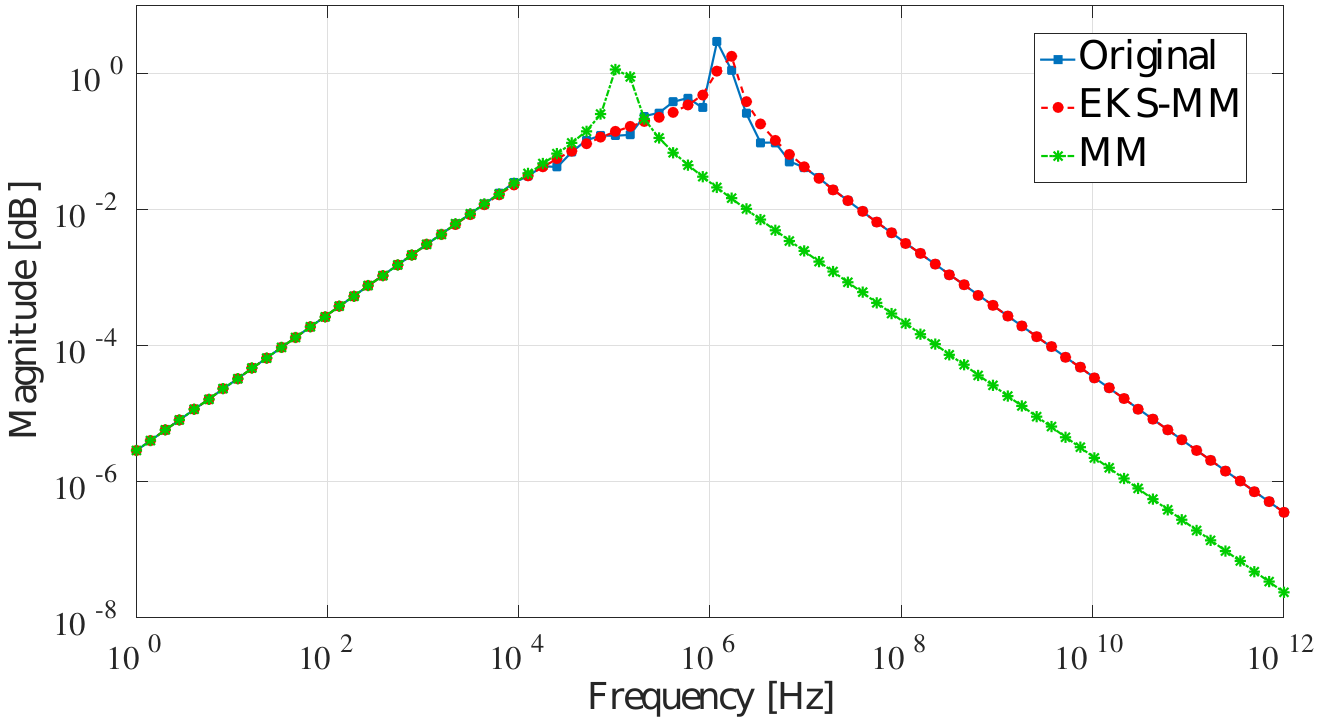
\includegraphics[width=\textwidth,height=\textheight,keepaspectratio]{FrequencyResponseAtPort9_9ofIbmpg1}
\end{figure}



\begin{figure}[h!]
\caption{Σύγκριση της συνάρτηση μεταφοράς στα υποβιβασμένης τάξης μοντέλα (\textlatin{Reduced Order Models (ROMs)} με τη χρήση της μεθόδου \textlatin{EKS-MM} και της κλασσικής μεθόδου \textlatin{MM} στο εύρος συχνοτήτων $[10^0, 10^{12}]$ για το αρχείο εισόδου \textlatin{ibmpg2t} για θύρες (4,4)}
\centering
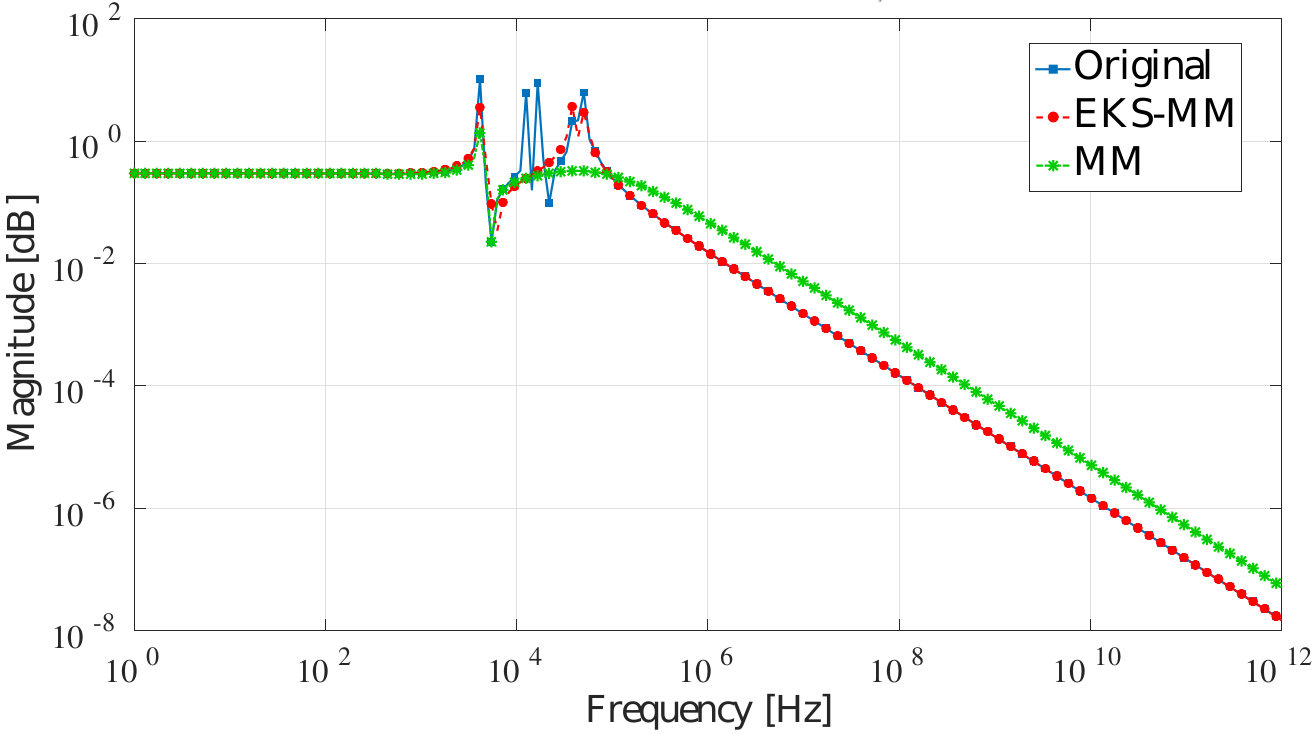
\includegraphics[width=\textwidth,height=\textheight,keepaspectratio]{FrequencyResponseAtPort4_4Ibmpg2t}
\end{figure}

\begin{figure}[h!]
\caption{Σύγκριση της συνάρτηση μεταφοράς στα υποβιβασμένης τάξης μοντέλα (\textlatin{Reduced Order Models (ROMs)} με τη χρήση της μεθόδου \textlatin{EKS-MM} και της κλασσικής μεθόδου \textlatin{MM} στο εύρος συχνοτήτων $[10^0, 10^{12}]$ για το αρχείο εισόδου \textlatin{ibmpg6} για θύρες (5,5)}
\centering
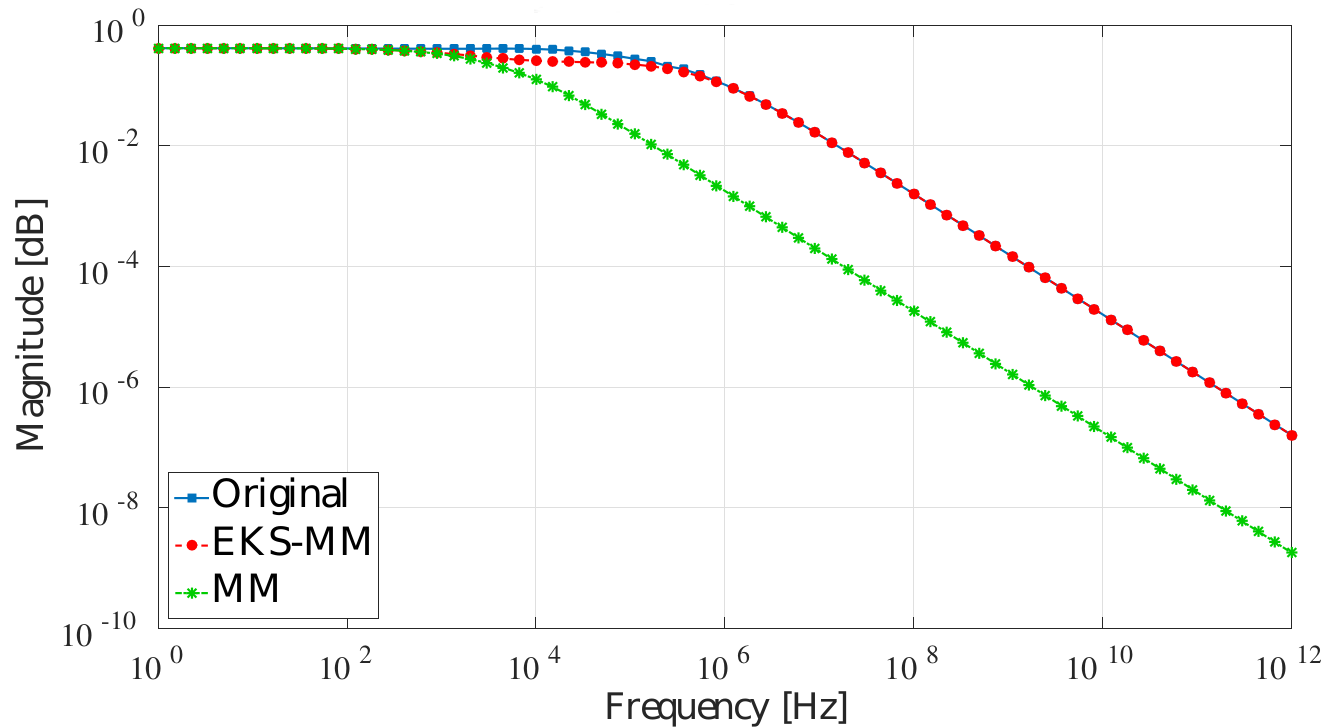
\includegraphics[width=\textwidth,height=\textheight,keepaspectratio]{FrequencyResponseAtPort5_5Ibmpg6}
\end{figure}

\begin{figure}[h!]
\caption{Μέγεθος του λάθους για τα υποβιβασμένης τάξης μοντέλα (\textlatin{Reduced Order Models (ROMs)} με τη χρήση της μεθόδου \textlatin{EKS-MM} και της κλασσικής μεθόδου \textlatin{MM} στο εύρος συχνοτήτων $[10^0, 10^{12}]$ για το αρχείο εισόδου \textlatin{ibmpg6} για θύρες (5,5)}
\centering
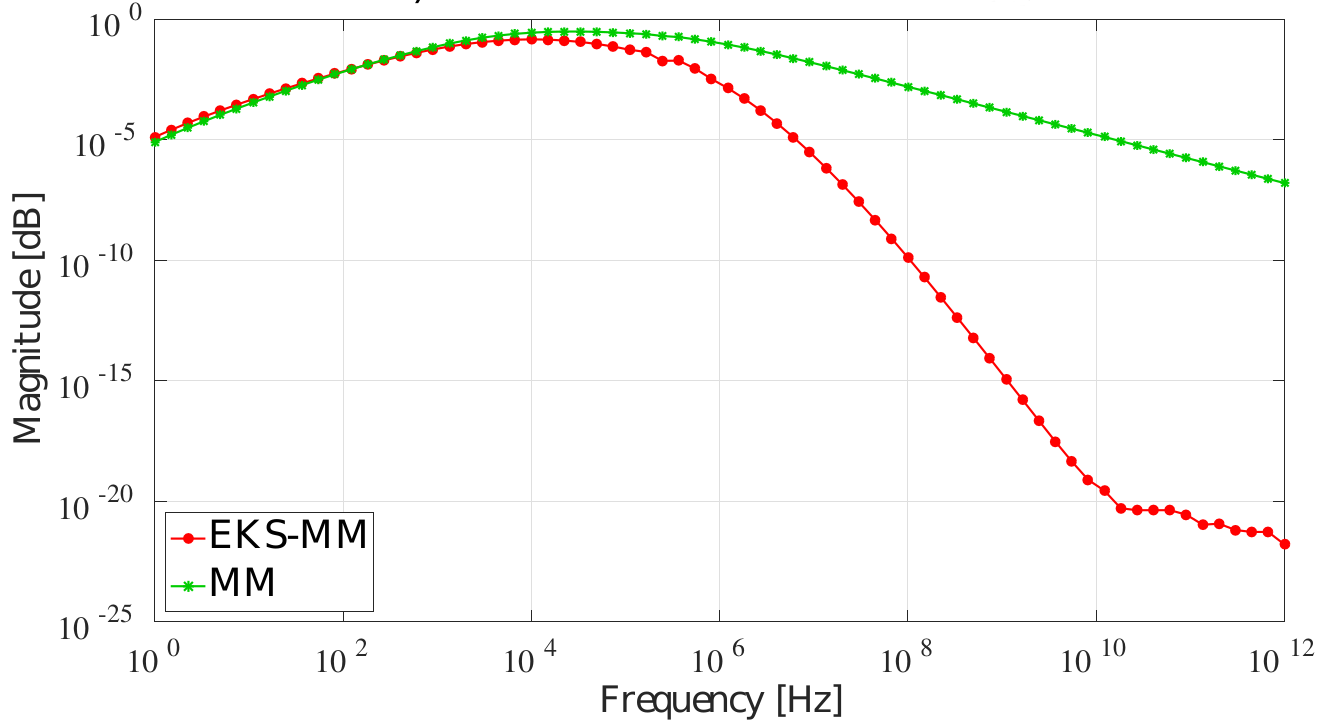
\includegraphics[width=\textwidth,height=\textheight,keepaspectratio]{MORErrorAtPort5_5Ibmpg6}
\end{figure}



\appendix
\chapter{Ακρωνύμια και συντομογραφίες}

\selectlanguage{english}
\begin{description}
  \item[MNA] Modified Nodal Analysis
  \item[KCL] Kirchhoff’s Current Law
  \item[SPD] Symmetric Positive Definite
  \item[MOR] Model Order Reduction
  \item[PRIMA] Passive Reduced-order Interconnect Macromodeling Algorithm
  \item[SPRIM] Structure-Preserving Reduced-Order Interconnect Macromodeling
  \item[MM] Moment Matching
  \item[ROMs] Reduced-Order Models
  \item[BA] Block Arnoldi
  \item[EBA] Extended Block Arnoldi
\end{description}
\selectlanguage{greek}

\include{chapterCSparse}
% \selectlanguage{greek}
% \chapter{Πειραματική Διαδικασία}
% \label{ch:chapterMatrixMarketFormat}

\selectlanguage{greek}
\chapter{Μορφή αρχείων εισόδου \textlatin{Matrix Market}}
\label{ch:chapterMatrixMarketFormat}

\section {Περιγραφή μορφής αρχείου}
Η μορφή αρχείων εισόδου \textlatin{Matrix Market} ~\cite{boisvert1996matrix} αποτελεί μια βασική μορφή απεικόνισης πινάκων σε μορφή \textlatin{ASCII} αρχείων. Το βασικό χαρακτηριστικό της μορφής αυτής είναι η απλότητα που τη διακρίνει κατά την περιγραφή ενός πίνακα. Ο στόχος της μορφής αυτής είναι να είναι εύκολα προσβάσιμο στη κατανόηση όσο από ανθρώπους όσο και από προγράμματα αλλά χωρίς να χάνεται η προσαρμοστικότητα σε εφαρμογές με πιο αυστηρές δομές ή η επεκτασιμότητα σε συναφείς δομές δεδομένων (όπως είναι η Τρίδυμη Δομή Απεικόνισης \ref{TripletForm} και Δομή της Συμπιεσμένης Στήλης\ref{CCS}).

Στα πλαίσια της παρούσας Διπλωματικής Εργασίας, θα εξετάσουμε δύο από τις βασικές μορφές δήλωσης πινάκων:

\begin{itemize}
    \item \textbf{Μορφή Συντεταγμένων \textlatin{Coordinate Format}} \\
    Είναι η βασική μορφή που χρησιμοποιείται για την αναπαράσταση αραιών πινάκων. Η μορφή αυτή περιλαμβάνει μόνο τις μη-μηδενικές τιμές μαζί με τις συντεταγμένες τους στον πίνακα. Όπως συμπεραίνουμε, η μορφή αυτή είναι ιδανική μόνο όταν τα μη-μηδενικά στοιχεία είναι λιγότερα από τα μηδενικά.
    \item \textbf{Μορφή Πίνακα \textlatin{Array Format}} \\
    Είναι η βασική μορφή που χρησιμοποιείται για την αναπαράσταση πυκνών πινάκων. Στη μορφή αυτή, παρέχουμε όλες τις τιμές (μηδενικές και μη-μηδενικές) σε μια προ διατεταγμένη (ανά στήλη) σειρά.
\end{itemize}

Τα αρχεία εισόδου που διαχειριζόμαστε στην υλοποίηση μας είναι της πρώτης μορφής. Παραθέτουμε ένα απλό παράδειγμα πως ένας αραιός πίνακας αντικατοπτρίζεται σε αυτή τη μορφή:

\begin{center}
\begin{tabular}{ c c c c}
 10 & 15 & 0 & 0 \\ 
 0 & 2.34 & 0 & 221 \\  
 1.32 & 0 & 0 & 23.324 \\
 0 & 0 & 0 & 98.58
\end{tabular}
\end{center}

Το παραπάνω παράδειγμα είναι από έναν γενικό αραιό πίνακα $4x4$ με πραγματικές τιμές.

Στη μορφή \textlatin{Matrix Market} το παραπάνω παράδειγμα θα παρουσιάζεται ως εξής:
\selectlanguage{english}
\begin{verbatim}
%%MatrixMarket matrix coordinate real general
%===============================================================
4  4  7
1     1   10
1     2   15
2     2   2.34
2     4   221
3     1   1.32
3     4  23.324
4     4   98.58
\end{verbatim}
\selectlanguage{greek}
Η πρώτη γραμμή του αρχείου περιλαμβάνει τον τύπο της μορφής του αρχείου. Στην συγκεκριμένη περίπτωση, σημειώνει ότι το αντικείμενο εντός του αρχείου αντιπροσωπεύει έναν πίνακα σε Μορφή Συντεταγμένων \textlatin{Coordinate Format} και οι τιμές που περιέχονται εντός του πίνακα είναι πραγματικές σε κανονική μορφή.

Υπάρχουν διάφορες παραλλαγές της παραπάνω μορφής που περιλαμβάνουν μιγαδικές αλλά και ακέραιες τιμές καθώς και μορφές που οι θέσεις από τις μη-μηδενικές τιμές περιγράφονται βάση προτύπου (\textlatin{pattern matrices}).

Επίσης, επιπλέον παράμετροι μπορούν να χρησιμοποιηθούν για να δηλώσουμε συμμετρίες στον πίνακα οι οποίες μπορούν να μειώσουν ριζικά το μέγεθος των δεδομένων. Τέτοιες παράμετροι είναι \textlatin{symmetric, skew-symmetric, Hermitian}. Στις περιπτώσεις αυτές μόνο οι τιμές για το κάτω τριγωνικό μέρος του πίνακα χρειάζεται να βρίσκονται εντός του αρχείου.

Στη συνέχεια, στο παραπάνω παράδειγμα βλέπουμε ότι η πρώτη γραμμή μετά τα σχόλια (τα οποία ξεκινάνε πάντα με τον χαρακτήρα \% στην αρχή) έχουμε μια γραμμή η οποία έχει τη μορφή:\\

\begin{center}
\begin{tabular}{ c c c }
 Αριθμός Γραμμών & Αριθμός Στηλών & Αριθμός Μη-Μηδενικών Στοιχείων
\end{tabular}
\end{center}

Η παραπάνω γραμμή μας βοηθάει στο να δεσμεύσουμε με ακρίβεια τον χώρο που θα χρειαστεί το πρόγραμμα μας για να αποθηκεύσει τον πίνακα. 

Στη συνέχεια, όλες οι υπόλοιπες γραμμές έχουν την ίδια μορφή η οποία είναι η εξής:

\begin{center}
\begin{tabular}{ c c c }
 Συντεταγμένη Γραμμής & Συντεταγμένη Στήλης & Τιμή
\end{tabular}
\end{center}

Κάθε μια τιμή που λαμβάνουμε από το αρχείο την τοποθετούμε εντός του πίνακα που έχουμε στην μνήμη.



\selectlanguage{english}

\bibliographystyle{IEEEtran}
\bibliography{IEEEabrv,references}

\end{document}